\documentclass[10pt,conference]{IEEEtran}
%\documentclass[a4paper,12pt]{article}
%\usepackage{algpseudocode}
\usepackage{cite,latexsym,times,epsf,amsmath,amssymb,amsfonts,graphicx}
\usepackage{epstopdf}
\usepackage{graphicx}
\usepackage{subfigure}
\usepackage{multirow}
\usepackage{algorithmic}
\usepackage{algorithm}
\usepackage{amsmath}
\usepackage{verbatim}
\usepackage{booktabs}
\usepackage{authblk}
\renewcommand{\algorithmicrequire}{\textbf{Input:}}
\renewcommand{\algorithmicensure}{\textbf{Output:}}
\renewcommand{\baselinestretch}{0.915}
%\renewcommand{\algorithmicforall}{\textbf{Foreach}}
%\renewcommand{\algorithmicendfor}{\textbf{}}


\begin{document}
\title{Leveraging White Spaces in Wireless Access Networks}
\author[1]{Pengfei Cui}
\author[2]{Yuanyuan Dong}
\author[1]{Hui Liu}
\author[1]{Dinesh Rajan}
\author[2]{Eli Olinick}
\author[1]{Joseph Camp}
\affil[1]{Department of Electrical Engineering, Southern Methodist University}
\affil[2]{Department of Engineering Management, Information, and Systems, Southern Methodist University}
%\documentclass[10pt]{article}

%\usepackage{xkvltxp}


\maketitle


\begin{abstract}

Wireless mesh networks were previously thought to be an ideal solution for
large-scale Internet connectivity in metropolitan areas.  However, in-field
trials revealed that the node spacing required for WiFi propagation 
induced a prohibitive cost model for network carriers to deploy. The digitization 
of TV channels and new FCC regulations have reapportioned spectrum for data 
networks with far greater range than WiFi due to lower carrier frequencies. 
Also, channel occupancy of change the performance of wireless network across 
both ISM bands and white space bands. In this work, we consider how these white 
space bands can be leveraged in large-scale wireless mesh network deployments 
with in-field measured channel capacity. In particular, we present an integer 
linear programming model to leverage diverse propagation characteristics and 
the  channel occupancy of white space and WiFi bands to deploy optimal WhiteMesh 
networks. Since such problem is known to be NP-hard, we design a measurement driven 
heuristic algorithm, Band-based Path Selection (BPS), which we show approaches 
the performance of the optimal solution with reduced complexity.  We additionally 
compare the performance of BPS against two well-known multi-channel, multi-radio 
deployment algorithms across a range of scenarios spanning those typical for 
rural areas to urban areas. In doing so, we achieve up to 160\% traffic achieved 
gateways gain of these existing multi-channel, multi-radio algorithms, which are 
agnostic to diverse propagation characteristics across bands.  Moreover, we show 
that, with similar channel resources and bandwidth, the joint use of WiFi and 
white space bands can achieve a served user demand of 170\% that of mesh networks 
with only WiFi bands or white space bands, respectively. Further, through the 
result, we leverage the channel occupancy and spacing impacts on white mesh
network and study the general rules of band selection.



\end{abstract}

% Introduce the background and problem, claim contribution

\section{Introduction}
\label{sec:introduction}

% Background multiband networks, hetergeneous networks, vehicular applications
% Introduction of white spcae.
% Process:
% Clearify the channel in different cities
% Introduce 2 possible gain: 1. reduce # mesh nodes 2. given topology get average capacity 
FCC adopted rules to allow unlicensed radio transmitters to operate in the white space freed from TV band since 2010~\cite{fccwhitespace}. White space is popularly referred to unused portions of the UHF and VHF spactrum includes, but not limited to 54M-72MHz,76M-88MHz,174M-216MHz,470M-608MHz,and 614M-806MHz ~\cite{whitespacewiki}.
To use these band, FCC ruling requires white space devices(WSDs) to learn of spectrum availability at their respective locations from a database of incumbents. For example, in Dallas/Fort Worth, TX, 482M-488MHz band should be yielded for TV channels, in Chicago, IL 470M-482MHz band is reserved for TV channels. ~\cite{broadband}
 These bands provides superior propagation and building penetration compared to licensed ISM Wifi bands like the 2.4 and 5GHz bands, holding rich poetntial for expanding broadband capacity and improving access for wireless users.

% Wireless mesh networks
Wireless mesh network is able to provide broadband Internet access to large contiguous areas through less mesh nodes equipped with WSD due to the propagation characteristic of ISM bands. White space mesh is an economic way to provide backhaul internet service in rural area or other low density area employing the propagation characteristics.
White space could also be used to improve the urban or high density area connectivity through lower interference channels. 

Mesh deployment requires selecting the number and locations to place mesh nodes to cover the whole area and the nodes are inter-connected in order to access to Internet gateway points.
Unfortunately, prior white space mesh placement research fails to address the compatibility of current existing devices, for instance, iPhone, Mac Laptop do not have white space radios to access white space gateway points. For a realistic mesh network, the end hop to the client need to be able to work in ISM Wifi band. 
To appreciate the multiband mesh deployment problem, it is important to understand the differences between white spaces and the popular ISM bands where Wifi devices operate. First, in FCC rules, users in white space band have to yield primary users.Before enter a white space channel, users have to detect the channel occupation. Second, white space band may suffer some unknown interference such as wireless Mic. Such devices may turn on at anytime without warning. Third, white space is cleaner than ISM bands since most of the TV stations have stopped using the bands. And also since in white space is in lower band, the coverage of these band is larger than higher frequency ISM band which could help to reduce the mesh nodes. According to these advantages and disadvantages, the balance between white space bands and ISM bands is possible to provide imporvement of mesh network. 

% AP location estimate 

% Paper focusing
This work focus on minimize the mesh nodes when gurantee the coverage and connectivity of the network.
We present FIXME mesh node placement algorithms so as to minimize the deployed nodes, guarantee the coverage, and mesh node inter-connectivity.


% 

% Contribution
% problem/environment propose
% algorithms
% 
The main contributions of our work are as follows:
\begin{itemize}
\item We formulate the hetergeneous mesh node placement problem as a FIXME problem.  

\item We propose a methodology to leverage the infulence of white space in mesh networks.

\item We propose FIXME algorithms to minimize the numberof deployed mesh nodes.
% Also should we consider the cost of different kind of nodes (1 radio, 2 radios, 3 radios )

\item We perform extensive outdoor experiments from multiple environments and simulations to evaluate the proposed algorithms.


\end{itemize}



%The remainder of this paper is organized as follows. In Section II, we present the multiband adaptation problem and proposed algorithms. Section III discusses experimental evaluation of the multiband algorithms. We conclude in Section IV.


% Multiband architecture and interference model Linear optimization model, takinkg about frequency occupancy
\section{Problem Formulation}
\label{sec:problemformulation}

%\begin{table*}[t] 
\centering % centering table 
\begin{tabular}{|l|r|} % creating 12 columns 
\hline %\hline % inserting double-line 
% Entering 1st row 
$\alpha$   & Path Loss Exponent     \\
\hline % inserts single-line 
R & Communication Range \\
\hline % inserts single-line 
$I_r$ & Interference Range \\
\hline % inserts single-line 

\end{tabular} 
\label{tab:2channelcombination} 
\caption{Throughput achieved through Gateway nodes (Mbps) for various combinations of WiFi and White Space (WS) mesh topologies (Offered Load = 4 Mbps, Network Size = 30 mesh nodes).} % title name of the table 
\vspace{-0.1in}
\end{table*} 


% Organization of the Sec
In this section, we formulate the problem of how to optimally 
use WiFi and white space bands in concert when deploying wireless 
mesh networks.  We first describe our system model and illustrate 
the challenges of such a WhiteMesh architecture.  We then discuss
how to evaluate WhiteMesh networks and the corresponding goal of
both the optimization framework and the heuristic algorithm that 
we propose in the following section.  Finally, we present 
our integer linear programming model used to address the problem. 
 
\subsection{WhiteMesh Network Architecture}
\label{subsec:architecture}

%A node in ~\emph{Multiband Wireless Mesh Network} has limited multiple slots for installing radios working in different bands. 
%Two nodes share the same link should have a common channel. The sum of the loads on the links should 
% Explain propagation, factors of the environment and so on
Wireless propagation is the behavior of the signal loss characteristics 
when wireless signals are transmitted from a transmitter to receiver.
The strength of the receiving signal depends on both the line-of-sight
path (or lack thereof) and multiple other paths that are a result of 
reflection, diffraction, and scattering from obstacles in the 
environment~\cite{andersen1995propagation}. The widely-used Friis
equation characterizes the power of the received signal $P_r$ in terms 
of the power $P_t$ and gain $G_t$ of the transmitting signal, gain of 
the receiver $G_r$, wavelength $\lambda$ of the carrier frequency, 
distance $R$ from transmitter to receiver, and path loss exponent $n$ according 
to~\cite{friis}:
\begin{equation}
\label{eq:friis}
P_r=P_t+G_t+G_r+10n \log_{10}\left( \frac{\lambda}{4\pi R}\right)
\end{equation}
Here, the path loss exponent $n$ changes according to the
aforementioned environmental factors and ranges from 2 to 5 in typical
outdoor settings~\cite{rappaport}.


%The rules of radio propagation are complex and diverse
%such as the daily changes of environment, weather, and atmosphere changes due to cosmos activities.
%In most propagation models there are three basic propagation mechanisms: reflection, diffraction, and scattering ~\cite{andersen1995propagation}.
%For multiband mesh backhual network, the nodes are usually installed on the top of buildings or towers to get the best line of sight propagation. A line of sight propagation model is a reasonable hypotheses in wireless mesh network.
% propagation fomular, explain the band influence
%In popular \emph{Friis} propagation model, the received signal power of a node is represented as:
%\begin{equation}
%\label{eq:friis}
%P_r=P_t+G_t+G_r+10n log_{10}(\frac{\lambda}{4\pi R})
%\end{equation}
%
%Path-loss exponent \emph{$n$} is used to describe the environment factors, typically in outdoor environments range from 2 to 5.\cite{camp2006measurement}.
%In equation ~\ref{eq:friis}, in the specific environment with a common path-loss exponent and $P_t,G_t,G_r$ configuration, the received signal vary according to the band represented by wavelength $\lambda$.
%Since wireless radios have the same received signal threshold, lower frequency band could have a larger communication range $D_c$, and also a larger interference range $D_r$.

% Explain multiband vs multichannel
A common assumption in works that use many WiFi channels is that the
propagation characteristics of one channel is similar to another, 
since the channel separation is relatively small (e.g., 5 MHz for 
the 2.4 GHz band).
Many works which rely on such an assumption have focused on the 
allocation of multiple WiFi channels with multiple radios in 
multihop wireless networks~\cite{si2010overview}.  Here, a frequency 
band is defined as a group of channels which have
similar propagation characteristics.
%We use a similar assumption for %channels within a frequency band, but consider the propagation 
%differences of a channel in one band (e.g., 450 MHz) as compared to 
%another (e.g., 2.4 GHz). 
In this work, we consider the diverse propagation characteristics
for four frequency bands: 450 MHz, 800 MHz, 2.4 GHz, and 5.8 GHz.
We refer to the two former frequency bands as white space (WS) bands, whereas
we refer to the two latter frequency bands as WiFi bands.

Wireless mesh networks are a particular type of multihop wireless network
that are typically considered to have at least two
tiers~\cite{CRSK06}: {\it (i)} an access tier, where client traffic 
is aggregated to and from mesh nodes, and {\it (ii)} a multihop 
backhaul tier for connecting all mesh nodes to the Internet through 
gateway nodes. In this work, we focus on how to optimally allocate 
white space and WiFi bands on a finite set of radios per mesh node
along the backhaul tier, since we assume that client devices will use 
WiFi (due to the economies of scale).  In each of the WhiteMesh 
topologies studied in Section~\ref{sec:experimentdesign}, a sufficient 
number of orthogonal WiFi channels remain for the access tier to 
connect to clients using additional radios co-located on the mesh nodes.

\begin{figure}
\vspace{-0.0in}
\centering
\includegraphics[width=84mm]{figures/interferencerange2}
\vspace{-0.1in}
\caption{Example WhiteMesh topology with different mesh-node shapes 
representing different frequency band choices per link.}
\label{fig:interferencerange}
\vspace{-0.2in}
\end{figure}

% Make multiband challenges
Due to the broadcast nature of the wireless medium, greater levels of
propagation induce higher levels of interference.  Thus, in sparsely-populated
rural areas, the lower frequencies of the white space bands might be a
more appropriate choice for multihop paths to gateways having reduced hop
count. However, as the population and demand scales up (e.g., for 
urban regions), the reduced spatial reuse and greater levels of interference 
of white space bands might detract from the overall deployment strategy. In 
such urban areas, select links of greater distance might be the most 
appropriate choice for white space bands, especially since the number of 
available channels is often inversely proportional to the population (due 
to the existence of greater TV channels).
%The broadcast nature of the wireless medium makes it generate multiple access interference in wireless network.
%Employing White Space Band in lower frequency brings advantages for mesh network, 1) more orthogonal bandwidth reduce the contention and conflict in the network,
% 2) the propagation variation brings flexible topology by reducing connection hop counts in the network.
%However, at the same time, links in White Space Band also increase the interference range in the network making space reuse of the white space band channel difficult. 

Figure \ref{fig:interferencerange} depicts an example where mesh node $A$ 
could connect to mesh node $C$ through $B$ at 2.4 GHz, or directly connect 
to $C$ at 450 MHz. If 2.4 GHz were used, link $D,E$ might be able to reuse
2.4 GHz if they are out of the interference range. However, if link $A,C$
used 450 MHz, a lower hop count would result for the path, but lower levels
of spatial reuse also result (e.g., for link $D,E$). While the issues of 
propagation, interference, and spatial reuse are simple to understand,
the joint use of white space and WiFi bands to form optimal WhiteMesh 
topologies is challenge.

%To balance the larger communication range and interference range of white space band in mesh network is a key issue in ~\emph{Multiband Mesh Network} from ~\emph{Multiradio} scenario.

\subsection{Model and Problem Formulation}
\label{subsec:problem}

% Assumptions of the network
Our model is similar to prior multi-channel models~\cite{tang2005interference,
yuan2006cross,si2010overview}. However, in these models, different channels
have the same communication range $D_c$ and interference range $D_r$.  While
these works would attempt to maximize throughput in a multihop network topology
by an optimal channel assignment for a given set of radios, we hypothesize that
using radios with a greater diversity in propagation could yield overall network 
performance gains.  
% NEWClaim we consider we could use either multiple channels in a band and also multiple channels in different bands
Therefore, for a given set of radios, we allow the channel
choices to come from multiple frequency bands (i.e., multiband channel assignment, which also includes multiple channels in the same band).
To simplify the analysis, we assume the channel capacity of each band is equal.
In practice, we could easily calculate the proportional ratio of channels in 
each band according to their bandwidth.
We assume that the locations of mesh nodes and gateway nodes are given and
all mesh nodes have the same transmit power, channel bandwidth, and antenna gain.
Each mesh node operates with a classic protocol model~\cite{gupta2000capacity}. 

A mesh network could be represented by a unidirectional graph $G=(V,E)$, where
$V$ is the set of mesh nodes, and $E$ is the set of all possible physical links 
in the network. If the received signal (according to Eq.~\ref{eq:friis}) between 
two mesh nodes $i,j$ for a given frequency band (from the set of all bands $B$) 
is greater than a communication-range threshold, then a data link exists and 
belongs to the set $L$ with a fixed, non-zero capacity $\gamma$ according to the protocol 
model.  Correspondingly, a connectivity graph $C$ is formed for each 
band in $B$ such that $C=(V,L,B)$.  If the received signal for a given band is 
above an interference-range threshold, then contention occurs between
nodes.  We extend the conflict matrix in~\cite{tang2005interference} according to
different interference per band according to $F=(E_{i,j},I_{Set},B)$, where $E_{i,j}$
represents the link and $I_{Set}$ includes all the links are physically inside 
the interference range $D_r$ when operating on each band $b$.

%~\emph{Channel Assignment} is to assign radios between nodes in mesh network creating virtual links for network communication with minimum interference.
%Our objective is to get a channel assignment for a wireless mesh network formed by a set of static mesh nodes and wired gateway nodes. 
%Each node in the network is equipped with one or more radios could work in one of the permitted bands. 
%FIXME keep or not
%To clarify the ~\emph{White Space Band} influence, we assume radios in a node works in unique non-overlapping channels of multiple band, radios in two nodes share a common channel in the same band.
%We also assume all the nodes have the same transmitting power, antenna with the same gains and other configurations.
%To model the connectivity, we adopt classical ~\emph{Protocol Model} from Gupta ~\cite{gupta2000capacity}. If the received signal is above the threshold, the link would have a communication capacity, otherwise, the link could not exist.
%The interference exist as conflict contention when the received signal strength of other links are above the threshold; otherwise, the link will not be interfered by other links.

%The ~\emph{Gateway Nodes} and ~\emph{Mesh Nodes} locations are given. 
%In a network, ~\emph{Channel Assignment} naturally binds with a routing protocol for application, but have different target. We bind our model with a ~\emph{Shortest Path Routing} protocol for ~\emph{Channel Assignment} application and evaluation.
%Transmitting power, antenna gains, communication and interference threshold are given. From ~\emph{Friis Model}, we could get ~\emph{Communication Range} and ~\emph{Interference Range} of each  band. 
%Multiband multi-radio wireless network could be represented as an undirected graph $G=(V,E)$ according to the communication range and interference range. $V$ is noted as the nodes, and $E$ marked as the links in the network.

%The channel assignment is represented as ~\emph{Connectivity Graph}, $C=(V,L,B)$, $L$ denotes the set of links, $B$ denotes the set of frequency bands. 
%In protocol model, the channel capacity between two nodes in a channel is noted as $LC$. If the RSSI from a node to another node is above the threshold, $LC$ is a constant value, otherwise, it is zero. 
%
%We extend the ~\emph{Conflict Matrix} from Jain's work ~\cite{tang2005interference} with a flexible approach for interference,
% $CM=(E_{i,j},I_{Set},B)$. $E_{i,j}$ represents the link, $I_{Set}$ includes all the links are physically inside the interference range $D_r$. 

%Our model is similar to Multichannel Model in many previous works ~\cite{tang2005interference,yuan2006cross,si2010overview}. However, in Multichannel Model, the Communication Range $D_c$ and Interference Range $D_r$ of different channels in the same band have the same value. The Multichannel Model is unnecessary to consider the variation of communication and interference range due to band propagation.
%Multiband Channel Assignment work toward the same target as Multichannel Channel Assignment to provide richer connectivity with minimum interference with channel variation in more bands.

%The difficulty of the problem is that we can not know the interference before we assign channel to each node. Previous works have proposed ~\emph{Coloring, Cluster, Independent Set, Mixed Linear Integer} methodology to approach the solution of ~\emph{Multichannel Channel Assignment} ~\cite{mishra2005weighted,peng2012efficient,tang2005interference}. 
%However, these work fails to deal with the minimize hops and more frequency space reuse embedded in multiple bands scenario.
%Our work focus on multiband channel assignment 
%without explicitly considering network traffic/load ~\cite{marina2010topology}.
%We present a mixed linear integer model to understand the multiband scenario. We also analyze the relation between the ~\emph{Hop Counts} and ~\emph{Space Reuse}, then propose two heuristic algorithms approaching solution of this problem.

%\subsection{Evaluation Metric: Gateway Goodput}
%\label{subsec:metric}

Therefore, the problem we address is: to choose the connectivity graph $C$ which maximizes
the served user demand according to the throughput achieved through the gateway (defined below).
A key challenge is that selecting the optimal channels from
the set $B$ leads to a conflict graph $F$ which cannot be known {\it a priori}. Previous
works have proposed a coloring, cluster-independent set, mixed linear integer methodology
for a single band $b$~\cite{mishra2005weighted,peng2012efficient,tang2005interference}. However,
these works do not address a reduction in hop count or an increase in spatial reuse for a set of 
diverse bands $B$.  In particular, the goal of a network backhaul layer is to maximize 
the amount of mesh user demand served, which can be measured by the total goodput 
achieved through the gateways. Thus, to evaluate the 
performance of the multiband channel assignment, we use a performance metric of gateway goodput $X$, where:
\begin{equation}
\label{eq:goodput}
X=\sum_{w \in W, v \in V}T(w,v)
\end{equation}
Since the bottleneck of mesh network capacity has been shown to be the gateway's wireless 
connections~\cite{robinson2008adding}, gateway goodput considers all incoming and outgoing
wireless traffic $T$ onto the Internet. We describe the exact calculation of gateway goodput in 
Section~\ref{sec:experimentdesign} and consider gateway placement outside the scope of this work.

%is the traffic arrive at the gateway node and relay to the wired Internet. The good put performance is correlated with gateway placement, channel assignment and routing. 
%The calculation of ~\emph{Gateway Good put} is described in ~\ref{sec:experimentdesign} .Jointly optimization of channel assignment, gateway placement, and routing is out of the scope of this paper.


\section{In-Field Spectral Measurements}
\label{sec:measurements}

% How to motivate our measurements?
To characterize the spectral footprint of a representative and diversely-populated area, 
we perform spectral analysis measurements in the Dallas-Fort Worth metroplex. In this section, 
we discuss the experimental setup and quantify the measurement-driven spectral activity.
 
\subsection{Wardriving Experimental Design}
\label{subsec:measurementdesign}
We employ a Linux-based 802.11 testbed, which includes a Gateworks 2358 board with Ubiquiti XR radios 
(XR9 at 900 MHz, XR2 at 2.4 GHz, XR5 at 5.2 GHz) and a DoodleLabs DL475 radio at 450 MHz. We develop 
shell scripts which utilize tcpdump to enable the testbed to work as a sniffer, recording all 802.11 
packets. However, since the Gateworks platform only updates its estimate of received signal strength 
upon the reception of a new packet (and not all relevant channel activity is 802.11 based), we employ 
a spectrum analyzer to form a notion of inter-network interference with finer granularity.  Hence, we 
also use a Rohde \& Schwarz FSH8 portable spectrum which operates from 100 KHz to 8~GHz. The portable spectrum 
analyzer is controlled by a Python script on a laptop to measure the received signal strength.


% Quantify the measurements
% Inter network interference and quantification
% Intra network interference
% Interference
Interference is a key issue in wireless network design. Despite sufficient levels of received signal, 
interference can cause channels to be unusable (e.g., due to high levels of packet loss) or unavailable 
(e.g., due to primary users in cognitive radios)~\cite{haykin2005cognitive}. 
The interference in wireless networks could be divided into two categories according to the interfering 
source: {\it (i)} intra-network interference, caused by nodes in the same network, and {\it (ii)} 
inter-network interference, caused by nodes or devices outside of the network. 

We define an activity level to quantify the spectrum utilization. The activity level is the percentage 
of time which the interfering signal could impact an active wireless link. In practice, we use the sensing 
samples ($S_\theta$) above an interference threshold ($\theta$) over the total samples ($S$) in a time 
unit as the activity level ($A$) of inter-network interference:
\begin{equation}
\label{eq:actdef}
A=\frac{S_\theta}{S_a}
\end{equation}



% Clearify
To the best of our knowledge, there is no readily available mobile, multiband antenna from 450 MHz to 5.2 
GHz on the market. Thus, we use a 700-MHz mobile antenna to perform spectral analysis measurements. We then 
normalize the mobile antenna performance across bands with indoor experimentation. To do so, we use a 
Universal Software Radio Peripheral (USRP) N210 to generate signals at 450 MHz, 800 MHz, and 2.4 GHz. We 
feed the USRP signals directly to a spectrum analyzer and adjust the configuration of USRP to make the 
received signal strength in the receiver side the same as the 5.2 GHz signal from Gateworks 2358 with 
a XR5 radio. 
Then, we connect the signal source to a fixed multiband antenna (QT 400 Quad Ridge Horn Antenna) and 
measure the received signal at a fixed distance with the 700-MHz antenna. We compare the received 
signals from the antennas designed for each band with known gains to obtain the antenna loss for 
each band. We further adjust the received signal strength collected via the 700-MHz mobile antenna 
according to the normalization data set.

  \begin{figure}
  %\vspace{-0.0in}
  \centering
  \includegraphics[width=74mm]{figures/equipment}
  \vspace{-0.1in}
  \caption{Multiband Measurement Platform}
  \label{fig:equipment}
  \vspace{-0.3in}
  \end{figure}
  
% Duplicate measurement in WiFi
Our experimental platform is shown in Fig.~\ref{fig:equipment}. The mobile spectrum analyzer records 32 samples 
per second on each band under test with appropriate time stamps. The Gateworks sniffer platform also records all 
the received WiFi packets according to their time stamps. The duplicate samples in the WiFi bands reported by the spectrum analyzer 
and Gateworks are removed according to overlapping time stamps to calculate the activity level in the WiFi 
bands. The activity level of white space bands is calculated solely based upon the spectrum analyzer measurements 
since it is assumed that device operating in the white space bands is not yet 802.11 compliant.

Fig.~\ref{fig:drivemap} depicts a map of the FCC-approved white space channels with markers where we performed 
measurements in North Texas. To be representative of a broad range of community types, we consider populations of 
approximately 25 times one another according to the 2010 U.S. Census: Millsap (500), Weatherford (25K), and Dallas 
(1.25 M). We have collected measurements at multiple types of locations in Dallas, including a downtown area,
a residential area, and a university campus. In Weatherford and Millsap, we monitor wireless activities in three 
locations for 45 continuous minutes on a weekday in downtown, residential, and non-residential areas. Then, we 
post-process the data to calculate the activity level of each band at each location. First, we parse the SNR from 
the data logs via Perl scripts. Second, we merge the data from the two platforms according to their respective 
time stamps and calculate the activity level of each band across these locations. The activity level is then 
included in our framework as input parameter. 

\subsection{Highway Speeds to Fixed Locations} 
\label{subsec:measurementresult}
As an initial experiment, we perform a drive test from Dallas to Weatherford with cruise control set to 60 MPH while 
on the highway. The result of the in-field spectrum drive test is shown in Fig.~\ref{fig:drivetest} according to 
the location of the measurement. The measured activity via RSSI of 450 MHz is high in downtown Dallas and 
Fort Worth but has less spectral activity in the urban and rural area between these city centers. The low activity 
detected in the WiFi bands is due to the distance from the highway being typically larger than the propagation range 
of predominantly indoor wireless routers.

Our initial spectral analysis measurements agree with the the FCC restrictions (shown in Fig.~\ref{fig:drivemap}), 
greater spectrum utility by TV bands induce less spectral availability.
The drive test also shows that the spectrum 
utilization is roughly proportional to the population density in Fig.~\ref{fig:drivetest}. We use the measurements 
collected at fixed locations as marked on the map for the activity level calculation. 

\begin{figure}
%\vspace{-0.0in}
\centering
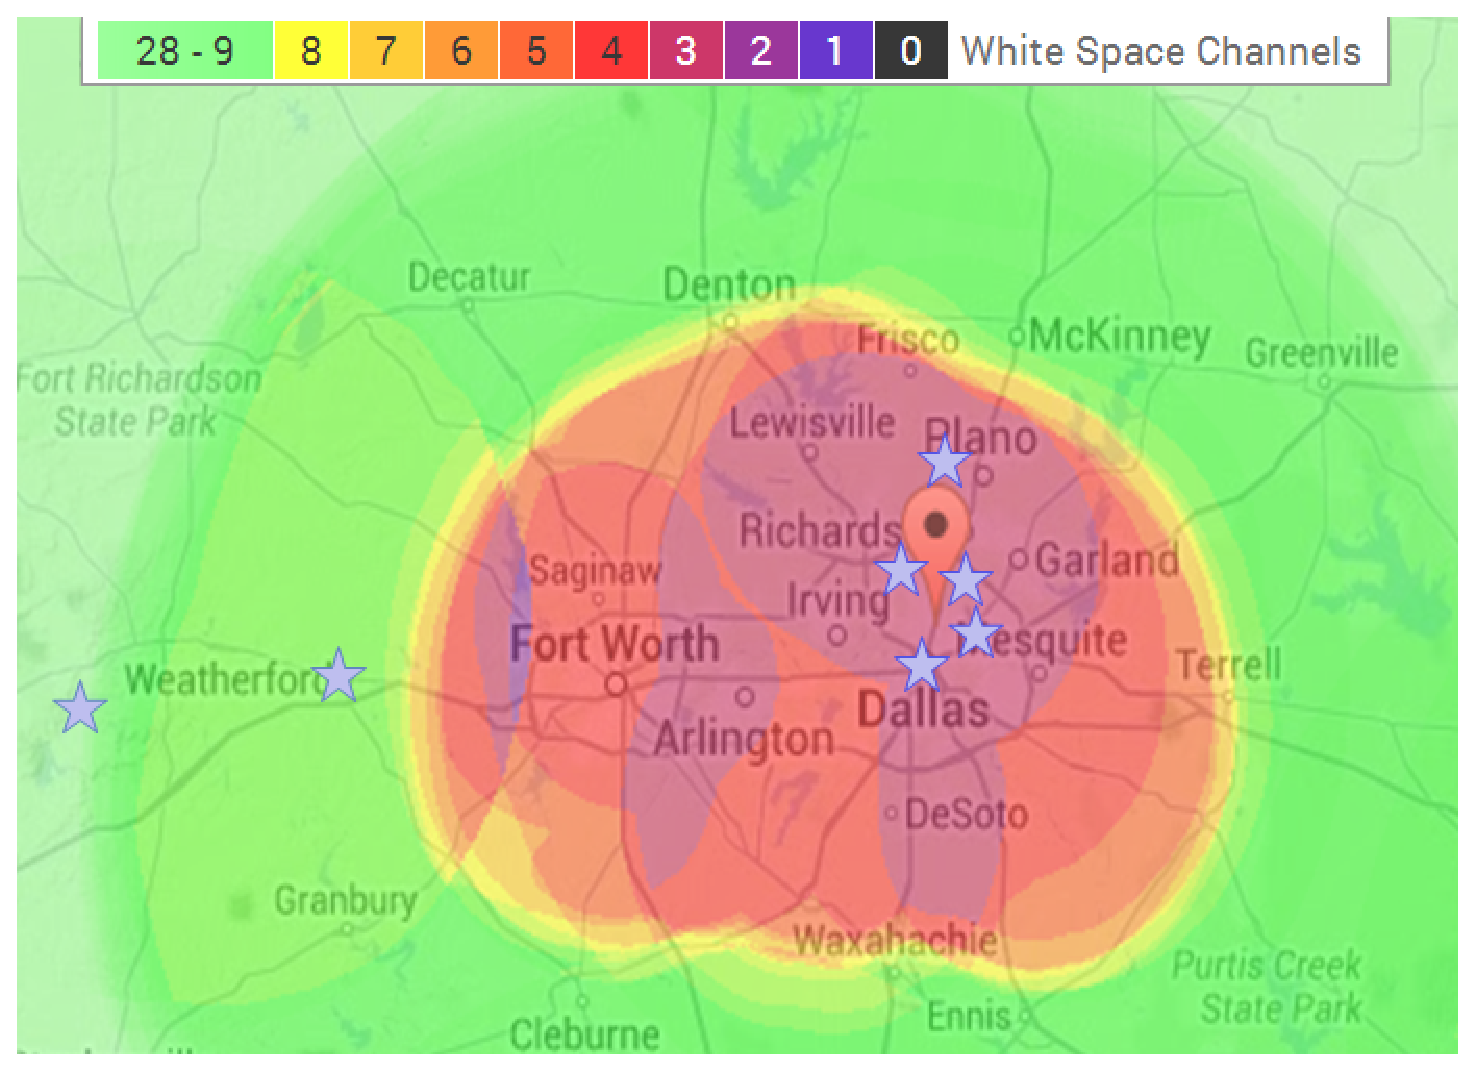
\includegraphics[width=74mm]{figures/drivemap}
\vspace{-0.1in}
\caption{White Space Channels in DFW Metropolitan and Surrounding Areas.}                                                                 
\label{fig:drivemap}
\vspace{-0.1in}
\end{figure}
   
\begin{figure}
%\vspace{-0.0in}
\centering
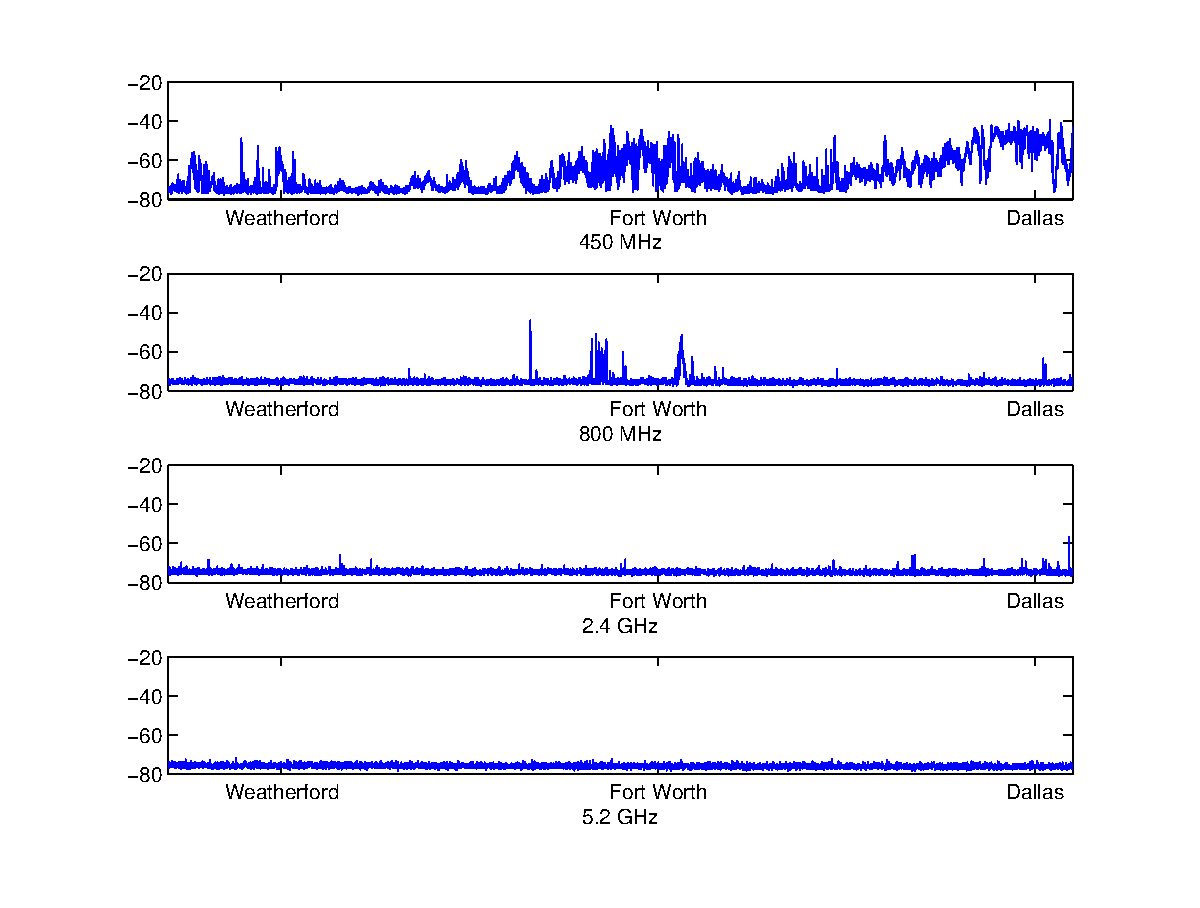
\includegraphics[width=84mm]{figures/drivetest}
\vspace{-0.3in}
\caption{Spectrum Activity in DFW Metropolitan and Surrounding Areas.}                                                                 
\label{fig:drivetest}
\vspace{-0.2in}
\end{figure}




% Here

The activity level calculated with our measurements are shown in Table~\ref{tab:activitymeasurement}. Dallas, the 
city with the greatest population in North Texas, has the highest activity level in most of the measured bands, 
especially at 450 MHz. The Dallas urban measurements are taken from the SMU campus, two neighborhoods, and a 
densely-populated suburb (Plano). Our measurements indicate that 2.4 GHz has a higher activity level in the aforementioned urban areas 
than the measured downtown area. Most schools and their neighborhoods are covered by WiFi, which contributes to the 
high activity level at 2.4 GHz and 5.2 GHz. In Weatherford, all the bands have lower activity levels than in Dallas. 
A peculiarity in the measurements can be seen by the sparse area in Weatherford having more activity than the other 
regions for 450 MHz. This can be explained due to the measurement location being on the East side of Weatherford (closer 
to Fort Worth, which has a population of approximately 750k). Millsap is a typical sparse rural area with approximately 
500 total residents. The activity levels across all the bands are lower than in Dallas and Weatherford. In the 450 MHz 
band, the activity level decreases much faster than in other bands in Dallas and Weatherford. 

\begin{table*}
\centering % centering table 
\begin{tabular}{|l|c|c|c|c|c|c|c|c|c|c|c|} % creating 12 columns 
\hline %\hline % inserting double-line 
Bands     & \multicolumn{3}{c|}{Dallas} & \multicolumn{3}{c|}{Weatherford} & \multicolumn{3}{c|}{Millsap} \\% [0.5ex]
\hline % inserts single-line 
% Entering 1st row 
Area Type & Downtown & Residential & Suburban & Downtown &  Residential & Sparse & Downtown & Residential & Sparse \\ % [0.5ex]
\hline % inserts single-line 
450 MHz &24.37	&25.83  &23.77	&6.05 &12.50  &14.03 & 7.00 & 0.07 & 0.02 \\      
\hline % inserts single-line                                                                                                       
800 MHz &4.40 	&16.49  &4.77	&5.22&5.07 &4.43  & 3.87 & 4.20 & 3.60 \\      
\hline % inserts single-line                                                                                                      
2.4 GHz &15.87 	&34.95  &2.60	&2.03&2.03 &2.77  & 2.07 & 1.60 & 0.80 \\      
\hline % inserts single-line                                                                                                     
5.2 GHz &19.70	&35.46  &1.53	&1.93&1.93 &1.33  & 1.27 & 2.07 & 2.10 \\      
\hline % inserts single-line 
\end{tabular}    
\caption{Activity Level in Multiple Locations} % title name of the table 
\label{tab:activitymeasurement}    
\vspace{-0.3in}
\end{table*}    


% Need a summary
Our measurements verify the channel occupancy variation in the DFW metroplex and quantify the occupancy
through a measurement-based activity level. The results show the spectrum bands have greater occupancy in
densely-populated areas. The measurements 
methods and resulting quantification provides the way to 
understand a typical deployment environment. We apply these 
measurements to our MAPE framework in Section.~\ref{sec:winmee} and BPS algorithms in Section.~\ref{sec:whitemesh} to 
further design access tier network deployments and backhaul tier multiband channel assignment, respectively.

\section{Access Network Deployment Algorithm and Evaluation}
\label{sec:winmee}

In this section, we study the access tier network deployment and propose our measurement-driven MAPE framework with the dynamics 
of WiFi and white space bands. We further apply our MAPE framework with the measurements shown in Section~\ref{sec:measurements}
to investigate the the access tier gain of WhiteMesh in reducing the number of access point in the Dallas-Fort Worth metroplex.

\subsection{Access Network Model and MAPE} 
\label{subsec:winmeemodel}


% Discuss the white space band in access and backhaul
% Traffic demand calculation
Access tiers must satisfy both the coverage and capacity constraints to provide service for users.
The coverage constraint could be calculated according to the propagation model of Eq.~\ref{eq:friis}. 
Generally, a coverage of $95\%$ of 
access tier is acceptable for wireless access networks~\cite{robinson2010deploying}. We represent the capacity 
constraint according to the demand of a service area, which could be calculated as the 
summation of individual demands all over the service area $D_a=\sum\limits_{p\in P} D_p$. Since household demand 
for the Internet has been previously characterized~\cite{rosston2011household}, $D_a$ could represent the 
population distribution $f$ and service area $k$ as $D_a=\sum\limits_{f \in F,k \in K}\bar{D_p}*f*k$. The capacity 
constraint could be represented with an access point set $M$ according to:
\begin{equation}
\label{eq:nlbound}
\sum_{m \in M}\delta_r^m \ge \sum_{f \in F,k \in K}\bar{D_p}*f*k
\end{equation}


% Discuss the application of activity level
Through the measured activity level, the achieved channel capacity could be calculated through the
free time according to:
\begin{equation}
\label{eq:intercap}
\delta_r=\delta*(1-\bar{A})
\end{equation}
Here, the capacity of a clean channel is denoted by $\delta$ under the protocol model. 
With the achieved channel capacity, we could further estimate the capacity of an access point in the access 
tier and link capacity in the backhaul tier.


In a joint white space and WiFi scenario, the activity level varies according to various interfering sources 
and the propagation characteristics induced by the environmental characteristics of the service area. A 
simple method with the least number of access points to cover an area is to use multiple orthogonal 
lower-frequency channels. However, the FCC limits white space band availability for data networks in most 
metropolitan areas in the United States~\cite{googledatabase}. Moreover, the number of channels in each band 
is limited. Too many lower-frequency channels will cause high levels of intra-network interference, 
which will be discussed in the next backhaul tier section. We assume that the cost of the network is proportional to the 
number of access points required for a given user demand (i.e., due to the cost of hardware and installation). 
Therefore, given a geographical region for a new network deployment, we build a measurement-driven framework 
called Multiband Access Point Estimation (MAPE) to compute the required number of access points.


\begin{algorithm}[t]
\small
\caption{Multiband Access Point Estimation (MAPE)}
\label{algorithm:mape}
\begin{algorithmic}[1]
\REQUIRE  ~~\\
$A$: Measured Activity Level \\
$F$: Population Distribution\\
$C$: Clean Channel Capacity\\
$n$: Path Loss Exponent \\
$B$: Available Frequency Bands\\
$M$: Area to be Covered
\STATE Split $M$ in to different type, calculate the traffic demand density $f$
\STATE Calculate in-field channel capacity $\delta_r$ as $\delta(1-A)$
\STATE Get the propagation coverage area radius $R_p$ from the Friis model based on $n,B,F$
\STATE Calculate the QoS coverage radius $R_{QoS}$ of a multiband access point that satisfies the demands of the area
\STATE The coverage radius of a multiband access point is $min\{R_p,R_{QoS}\}$
\STATE Apply a regular-hexagonal deployment to get the number of access points for serving given area $M$
\ENSURE ~~\\
The number of access points\\
\end{algorithmic}
\end{algorithm}

In the spatial domain, the advantage of higher-frequency channels is the spatial reuse, while the lower-frequency 
channels provide greater levels of coverage. Generally, higher frequencies are more appropriate for populated 
areas, and lower frequencies are more appropriate for sparse areas. The temporal variation of spectrum utilization 
differs across bands. For an Internet service provider, the service quality which maps to the capacity constraint 
must be satisfied. Given a metropolitan area, the population distribution can be found according to census data~\cite{uscensus}. 
Then, we can estimate the capacity demand of each type of area with the assumption that users 
will exhibit average demand. According to the population distribution, we split the area into different types,
which compose the spatial input. Then, we use the measured activity level as the temporal input. We have an average 
channel capacity of each band according to the activity level. With the received signal strength threshold, the 
Quality-of-Service-constrained coverage area of different types per channel, and the spatial reuse distance can be 
directly computed. Then, the maximum area an access point could cover can be calculated as the minimal area of the 
QoS-based coverage area and propagation coverage. Then, the transmission power is adjusted to fulfill the coverage 
restriction subject to the FCC regulations for maximum-allowable transmit power. A regular-hexagonal deployment 
process is employed to place the access points. 

\subsection{Results and Analysis}
\label{subsec:winmeeresult}

We use the measurement-based activity levels shown in Table~\ref{tab:activitymeasurement} as an input to 
Alg.~\ref{algorithm:mape}. We specifically use the Millsap sparse area, Millsap downtown, Weatherford residential, 
Dallas residential, and Dallas downtown measurements as inputs of activity level for a given population density. We then 
calculate the number of access points for covering a 13 km $\times$ 13 km area, varying the population density. The 
output is shown in Fig.~\ref{fig:redensity}. 

   \begin{figure}
   %\vspace{-0.0in}
   \centering
   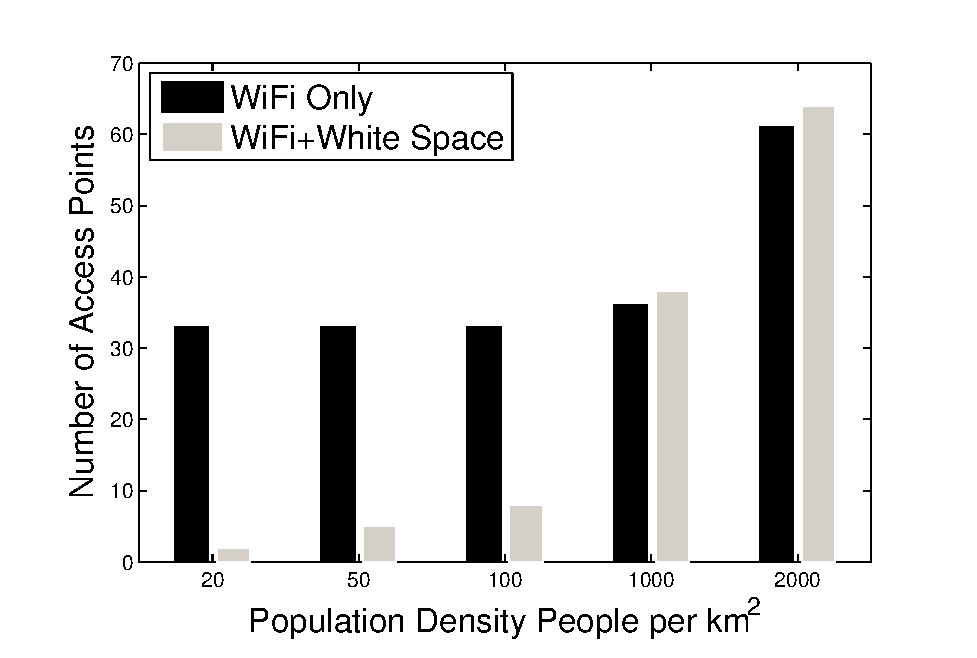
\includegraphics[width=84mm]{figures/redensity}
   \vspace{-0.1in}
   \caption{Number of Access Points Needed for a 13 km x13 km Area.}
   \label{fig:redensity}
   \vspace{-0.3in}
   \end{figure}

% Experiment Results & expect results
In the calculation, we set the demand requested per user to be 2 Mbps with the population density of 20, 50, 100, 1000, 
and 2000 users per square kilometer. We assume 30\% of the residents will use this service (i.e., the take rate is 
30), the maximum transmit power is 30 dBm, with a path loss exponent of $3.5$~\cite{meikle2012global}. From Eq.~\ref{eq:friis}, 
we see that the propagation range is proportional to the wavelength with 450 MHz having a propagation 
range of $11.6$ times that of 5.2 GHz. We adopt an 802.11n maximum data rate of 600 Mbps. For the WiFi+White Space 
scenario, we use 3 channels in each of the 450 MHz, 2.4 GHz and 5.2 GHz bands. For the WiFi Only scenario, we assume 
6 channel in the 2.4-GHz band, and 3 channels in the 5.2-GHz band since 2.4 GHz has a greater propagation range than 5.2 GHz. 
Each of these scenarios have the same channels in total (9). As shown in Fig.~\ref{fig:redensity}, with the same number 
of channels, the WiFi+White Space scenario reduces the number of access points by $1650\%$ compared to the WiFi Only scenario in the 
20 people per square km scenario, $660\%$ in the 50 people per square km, and $412.5\%$ in the 100 people per square km 
scenario. The large propagation range of the white space bands is approximately 10 times that of the WiFi bands, creating 
an opportunity for greater coverage. However, as the population density increases, due to the capacity constraint of 
servicing users in the area, the lower-frequency white space bands lose their advantage of larger communication range due 
to the reduction in achievable spatial reuse. At the same time, the activities of other signal sources, such as TV stations 
in downtown areas, reduce the capacity of white space bands. As a result, the WiFi+White Space scenario performs worse 
than the WiFi Only scenario. If we were to count the intra-network interference as in the following section, the situation could become 
even worse. Moreover, FCC has stricter policies on white spaces in urban areas. Fewer channels are available in the 
downtown and urban areas, which makes WiFi a better option for these dense areas.

To understand the influence of band combinations on network deployments, we calculate the number of access points in the 
area when selecting 500 people per square km with a downtown Weatherford spectrum utilization and 1500 people per square 
km with a residential Dallas spectrum utilization. We assume the total number of channels is 12. We use the same setup 
as the previous experiment.
 
 \begin{table}[h]
 \centering
 \begin{tabular}{|c|c|c|c|}
 \hline
 \multirow{2}{*}{No. of Bands} & \multirow{2}{*}{Bands Combination} & \multicolumn{2}{c|}{No. of AP} \\
 \cline{3-4}
  &  & 500 & 1500 \\
 & (Hz) & $ppl/km^2$ &  $ppl/km^2$ \\
 \hline
 \multirow{4}{*}{1}    & 450 M  & 12  & 35 \\
 \cline{2-4}
                              & 800 M & 10  &  30 \\
 \cline{2-4}
			      & 2.4 GHz & 33  &  37 \\
 \cline{2-4}
                              & 5.2 G & 193 &  193 \\ 
 \hline
 \multirow{6}{*}{2}   & 450 M,800 M & 11  & 32\\
 \cline{2-4}
                              & 450 M,2.4 G & 23  & 36\\
 \cline{2-4}
			      & 450 M,5.2 G & 23  & 69\\
 \cline{2-4}
			      & 800 M,2.4 G & 20  & 33\\ 
 \cline{2-4}
			      & 800 M,5.2 G & 20  & 59\\ 
 \cline{2-4}
			      & 2.4 G,5.2 G & 33  & 73\\ 
 \hline
 \multirow{4}{*}{3} & 450 M,800 M,2.4 G & 16  & 33\\
 \cline{2-4}
                              & 450 M,800 M,5.2 G & 16  & 48\\
 \cline{2-4}
			      & 450 M,2.4 G,5.2 G & 33  & 53\\
 \cline{2-4}
			      & 800 M,2.4 G,5.2 G & 30 &  49\\ 
 \hline
 4  & 450 M,800 M,2.4 G,5.2 G & 21  & 44 \\
 \hline
 \end{tabular}
 \caption{Channel Combinations for $500$ and $1500$ Population Density Scenarios}
 \label{tab:500comb}
 \vspace{-0.4in}
 \end{table}


In Table~\ref{tab:500comb}, we compare the number of access points with 12 channels through all 
the possible combinations of bands. 
% Single band compare
Since purchasing and deploying access points is the primary cost of a wireless 
infrastructure, to simplify the calculation, we only count the number of access points as 
the network's cost. 
When all the channels are in the same band, as the frequency goes up, more access 
points are needed to serve the area due to the limited propagation range. However,
450 MHz does not outperform 800 MHz with a single band at both the 500 and 1500 people per
square km cases because 450-MHz channels have larger measured activity levels. 
White space band channels outperform WiFi bands by up to 1830\% in the single band case
with 500 people per square km, but with 1,500 people per square km, the cost reduction
decreases to only 543\%.
% Two bands 
We now distribute an equal number of channels to two-band combinations and run the experiments 
with the same population densities and spectrum utilization. The results show that the white space band
combination (450 and 800 MHz) performs better than WiFi only (2.4 and 5.2 GHz) by 200\% and
128\% with the people per square km of 500 and 1,500, respectively. In fact, the white space only
scenario (450 and 800 MHz) has almost the same performance as the scenarios with one white band and
one WiFi band (450 MHz and 2.4 GHz; 800 MHz and 2.4 GHz) with 1,500 people per square km.
However, with 500 people per square km, the white space only scenario is much better than any other two-band combination.
% Three bands
White space channels provide up to 87.5\% cost reduction in three-band combination scenarios with
500 people per square km, and up to 33.3\% with 1,500 people per square km.  With four bands,
the number of access points required does not reduce using white space bands.

From Fig.~\ref{fig:redensity} and Table~\ref{tab:500comb}, we show that as the population
density increases, the reduction in number of access points required to meet the same demand 
diminishes. Note that a more optimal allocation of channels in different bands could offer
further cost reductions. We further show that as population and spectrum utilization increase, 
at some point, the performance of white space only scenario could be the same as a combination of
white space and WiFi bands. 


\section{Backhual Algorithm and Evaluation}
\label{sec:whitemesh}

% Organization of the Sec
In this section, we study the channel assignment problem jointly when using WiFi and white space 
bands in concert across the backhual tier of a wireless mesh network. We then present our linear programming model and 
heuristic-based measurement-driven algorithm to address the problem. 
 
\subsection{Linear Programming Formulation}
\label{subsec:linearopt}

The function of the backhual tier is to wirelessly provide end to end traffic to and from the user and Internet.
% Metrics
In practice, the traffic demand of the users obeys a Poisson process~\cite{saaty1961elements}. 
Most of the carriers charge users based on the traffic being tranferred oner the Internet. 
The traffic demand of the users delivered to or from the Internet are noted as the total traffic served. 
In particular the total traffic served $X$, is represented as:
\begin{equation}
\label{eq:goodput}
X=\sum_{w \in W, v \in V}T(w,v)
\end{equation}
$T(w,v)$ nodes all delivered traffic between access point $v \in V$ and gateway node $w \in W$.

%To clarify the problem and approach the optimization solution of the problem, 
Here, we present a linear programming formulation to approach the optimal channel assignment in along the backhaul 
tier of a WhiteMesh network. 
We leverage the nodes into consider the set of available access points ($V$) which aggregate the traffic from the users, 
and gateways ($W$) as ingress points to the Internet. The available frequency bands ($B$) are pre-known 
as an input. The conflict graph $I$ is given as parameters. 
$\delta_b$ is the achieved channel capacity estimated from the  activity level measurements 
introduced in Section.~\ref{sec:measurements}.


\noindent
{\bf Sets:}
\begin{tabular}{ll}
$V$ & set of nodes \\
$B$ & set of bands \\
\end{tabular}

\noindent
{\bf Parameters:}\\
\\
%\vspace{0.1in}
%\begin{tabular}{lll}
\begin{tabular}{llp{3.4cm}}
%\hline
$\delta^b$ & $b \in B$ & Achieved capacity of band $b$ in target area\\
%\begin{tabular}{llp{2.8cm}}
$I_{ij,lm}^b$ & $(i,j,l,m) \in V, b\in B $ & Protocol Interference of link $(i,j)$ on band $b$ brought by link $(l,m)$\\
%\hline
%\end{tabular}\\
%\begin{tabular}{llp{2.8cm}}
$W_i$ & $i \in V\ binary$ & Gateway marked with access point set\\
%\hline
%\end{tabular}\\
%\begin{tabular}{llp{2.8cm}}
$D_{d}$ & $i \in V\ $ & Downlink demand of node i\\
%\hline
%\end{tabular}\\
%\begin{tabular}{llp{2.8cm}}
$D_{u}$ & $i \in V\ $ & Uplink demand of node i\\
%\hline
\end{tabular}

The variable time share $\alpha_{i,j}^b$ represents the assigned percentage of a single link transmitting time  
for link $i,j$ between node $i$ and node $j$ in band $b$. 
The two variables, $uy_{i,j,k}^{b}$ and $dy_{i,j,k}^{b}$ are defined as uplink and downlink flows:

\noindent
%\vspace{2pt}
{\bf Variables:}\\
\\
%\vspace{1pt}
\begin{tabular}{llp{3cm}}
$0\le \alpha_{ij}^b \le 1$  & $b\in B, (i,j) \in N$ & 
Time share of link $(i,j)$ on band $b$\\ 
$0\le uy_{i,j,k}^b$ & $(i,j,k) \in V, b \in B$ & 
Uplink flow of node $k$ on link $(i,j)$ at band $b$ \\ 
$0\le dy_{i,j,k}^b$ & $(i,j,k) \in N, b \in B$ & 
Downlink flow of node $k$ on link $(i,j)$ at band $b$ \\ 
\end{tabular}
\vspace{1pt}

% FIXME talk about NT calculation
The objective is to maximize the total traffic served ($X$) of all the gateways, $X$ is defined in Eq.~\ref{eq:goodput}.
It is represented with the variables:

\noindent
{\bf Objective:}
\begin{align}
& Max \sum_i\sum_j\sum_k\sum_b(uy_{i,j,k}^b+dy_{j,i,k}^b) \;\ When \; w_j=1 
%& Max \sum_i\sum_j\sum_b(\frac{1}{\sum_{l,m}\alpha_{i,j}^b\times I_{ij,lm}})
\end{align}

In this LP formulation, the constraints are presented as connectivity, uplink, and downlink sections here:  

\noindent
%{\bf Constraints:}
{\bf Connectivity Constraints:}
\begin{align}
\label{opt:1}
& \alpha_{i,j}^b + \alpha_{j,i}^b + \sum_l\sum_m(\alpha_{l,m}^b \cdot I_{ij,lm}^b) \leq \delta^b, i\neq j \\
\label{opt:2}
& \sum_i uy_{i,j,k}^b + \sum_i dy_{i,j,k}^b \leq \delta^b \cdot \alpha_{j,k}^b 
\end{align}
\noindent
{\bf Uplink Constraints:} 
\begin{align}
\label{opt:3}
& \sum_k \sum_b uy_{i,k,i}^b \leq D_{ui}  \; ; w_k=0, i \neq k \\
\label{opt:4}
& uy_{i,j,k}^b \cdot w_k = 0 \\
%\label{opt:5}
%& \sum_i\sum_b uy_{i,j,k}^b - \sum_m\sum_b uy_{j,m,k}^b = 0 \; when \; w_k=0, i\neq k\\
\label{opt:6}
& \sum_{i\neq j}\sum_b uy_{i,j,k}^b = \sum_{m\neq j} \sum_b uy_{j,m,k}^b \; ;w_j = 0\\
\label{opt:7}
& uy_{i,j,i}^b=0 
\end{align}
\noindent
{\bf Downlink Constraints:} 
\begin{align}
{\bf}
\label{opt:8}
& \sum_k \sum_b dy_{i,k,i}^b \leq D_{di} \; \; ; w_k=0 \\
\label{opt:9}
& dy_{i,j,k}^b =0  \; ;w_k=1 \\
%\label{opt:10}
%& \sum_j\sum_b dy_{i,j,k}^b - \sum_m\sum_b dy_{i,k,m}^b \geq , i \neq k \\
\label{opt:11}
& \sum_{i\neq j} \sum_b dy_{i,j,k}^b = \sum_{m \neq j} \sum_b dy_{j,m,k}^b   \; ; w_j=0, i \neq k \\
\label{opt:12}
& dy_{i,i,j}^b=0
\end{align}

In these constraints, (\ref{opt:1}) represents the total time assigned for the incoming flows, outgoing flows, 
and the interfering time which should all be less than 1. Constraint (\ref{opt:2}) represents that the incoming and 
outgoing wireless traffic are less than the capacity assigned for link $i,j$. Uplink constraints 
(\ref{opt:3}) and (\ref{opt:4}) represent that the total traffic flow on link $i,j$ from $i$ is less than 
the demand of node $i$. Constraints (\ref{opt:6}) and (\ref{opt:7}) restricts the sum of incoming data 
flows for a given access point $k$ equal to the total outgoing flows from the node. Downlink constraints 
(\ref{opt:8}) and (\ref{opt:9}) represent similar restrictions as (\ref{opt:3}) and (\ref{opt:4}), but 
in the downlink direction. Similarly, constraints (\ref{opt:11}) and (\ref{opt:12}) are downlink versions of 
(\ref{opt:6}) and (\ref{opt:7}).
Since linear programming models for multiple channels has been proved to be NP-hard~\cite{yuan2006cross},
in this work, we choose small set of cases to achieve the optimal solution.



% PEN part 
%% Talk about the network efficiency for multiband multihop mixed hop

In ~\emph{Multiband Multiradio Network}, 
a multihop path could have higher frequency band combination with less interference range or a set of lower frequency band with less hop count.
A key issue of multihop path in such network is to answer which combination is better.
We focus our work on ~\emph{Channel Assignment} dealing with more interference factors rather than routing protocol which would be more concern on delay. Other architecture also has such problem such as wireless sensor network.

To discuss this problem, we pick up a multihop path from mesh network and analyze its performance with worst case hypothesis. In mesh network, such a path would have a bottle neck in the link closet to gateway.
When a mesh network was built with gateway placement, constructor should considered load-aware demand of mesh nodes and mesh node population. 
Generally the nodes close to gateway should have more traffic demand and gateway itself should have the most connectivity population. 
We treat each node equally binding with fairness, otherwise mesh nodes close to gateway could be served more traffic and show a high goodput of the network.
For analyze, we assume all the node in the path equally share the time of the link next to a gateway. It is also the worst case for getting a larger goodput.


First, we introduce the ~\emph{Intra-Path} traffic. When we have a multihop path, in worst case all the nodes on the path have only one $h$ hop path arrived at a gateway node. The path is made of links from one node to another.
Each node has traffic $T$, nomatter uplink or downlink since both of them occupy link capacity in the same way. And the total traffic on the path $\sum T$ is less than the bottle neck link capacity $C$. 

We define the minimum transmission rate on a path as ~\emph{Network Efficiency}. 
With the fairness restriction, the last node in the path has the minimum transmission rate.
Then the acitve time in a time unit of each link can be represented as $1,\frac{h-1}{h},\frac{h-2}{h}\cdots \frac{1}{h}$. 
The unit time of each link in the path is counted as total cost time of network.
%\begin{equation}
%\label{eq:intrapath}
%\begin{split}
%E_{Intra-Path}=\frac{Path\ Active\ Time}{Network\ Time}\\
%E_{Intra-Path}=\frac{1}{2}+\frac{1}{2\cdot h}
%\end{split}
%\end{equation}


%As hop count increase, the ~\emph{Intra-Path} will decrease till the lower bound $\frac{1}{2}$. With routing protocol which is out of this work, the delay increase too.
Without considering ~\emph{Inter-Path} interference which represent interference with links out of the path, 
an intuition of using lower band is to reduce the hop count
 to increase the minimum time utility rate which is the active time of the last link over the total active time of the path. 
However, at the same time, the interference range increase too. An example shown in ~\ref{fig:networkefficiency}, 
the picture shows links in different bands, let's say 2.4GHz and 900MHz, as a sketch map, does not represent the real distance.
Node $A,C$ could be connected through two 2.4GHz links or a single 900MHz link; with 2.4GHz links, only link $D,E$ will be interferenced; however, with 900MHz $A,C$ link, link $F,G;M,L;K,J$ will be interferenced. 


\begin{figure}
%\vspace{-0.0in}
\centering
\includegraphics[width=74mm]{figures/networkefficiency}
\vspace{-0.1in}
\caption{Path Network Efficiency Introduction, Solid Wire notes 2.4GHz link, Dashed line notes 900MHz}
\label{fig:networkefficiency}
%\vspace{-0.0in}
a\end{figure}

To quantization this ~\emph{Inter-Path Interference}, 
the unit time of these links are counted as ~\emph{Network Time}. 
When a $h$ hop path transmitting traffic $T$ for the destination node, it stops activity on a number of links in the same band. 
In a multihop path, when the traffic arrived at the last destination node, all the previous links are serving for these traffic.
The active time on a single link can be noted as 
$\frac{T}{c_h}$. We keep in the worst case when the last node in the path got traffic $T$, the other node also be served traffic $T$.
With interference counts $I_h$ from the conflict matrix:
the ~\emph{Network Time} counted as 
$\frac{hT}{c_1}\cdot I_1 + \frac{(h-1)T}{c_2}\cdot I_2 \cdots \frac{T}{c_h}\cdot I_h$, the ~\emph{Path Efficiency over Network} is defined the traffic over the ~\emph{Network Time} and could be represented as:



\begin{equation}
\label{eq:originpen}
E_{PEN}=\frac{T}{\sum_{i \leq h}\frac{i\cdot T}{c_h}\cdot I_i }
\end{equation}

With protocol model, if link exist, then they have the same capacity $c_1=c_2 \cdots =c_h=c$. 
To avoid $0$ value in the denominator, we add a $1$ to adjust the denominator which does not change the parameter characteristics. 
The \emph{Path Efficiency over Network}could be represented as:


\begin{equation}
\label{eq:pen}
E_{PEN}=(\frac{c}{1+\sum_{i \leq h} i\cdot I_i}
\end{equation}
 

The meaning of the ~\emph{Network Efficiency} is that in a unit time, the traffic could be loaded by this path. In multichannel scenario, all the channel will have the same communication range, this parameter equals to the conflic graph in many multichannel works which try to minimize the interference~\cite{jain2005impact}. Since we count only one channel not all possible links, it also could be seen as an extention of a single link ~\emph{Link Load} defined in ~\cite{raniwala2004centralized}.

The ~\emph{Path Efficiency over Network} connect hop counts and interference. 
Then we discuss when a lower ~\emph{White Space Band} is better to be used in a path.
In a path, we use an average interference count $\bar{I}$ replace each interference count with assumption the links in the path all in one higher freq band. Then a ~\emph{White Space Band} is used to replace two links in the path as a single link with interference count $X$ represent one of the factor $i\cdot I_i$. The problem could be formulated as:

 
\begin{equation}
\label{eq:benefit}
\frac{c}{1+\frac{h(h-1)}{2}\cdot \bar{I}+X} \geq \frac{c}{1+\frac{h(h+1)}{2}\cdot \bar{I}}
\end{equation}

From the inequation, when $X \leq 2\cdot h\bar{I}$ a lower band could be better. $X$ is also a function of hop order in the path, generally the path order lower, the threshold would be more strict; otherwise it could be loose. It matches the intuition the hop order is small, it close to the gateway, it should be more crowd for this link.
It helps to tell the ranking of set of links and a path where we can start to resolve channel assignment problem.









\subsection{Path Interference Induced on the Network}
\label{subsec:PEN}

In WhiteMesh networks, it is possible that multihop paths are intermixed with WiFi bands for more spatial reuse 
and white space bands with hop count reduction. We analyze the band choices reducing the number of hops along 
a path and the aggregate level of interference on that hop-by-hop path choice has on the network (i.e., Path 
Interference induced on the Network).

Mesh nodes closer to the gateway generally achieve greater levels of throughput at sufficient-high 
offered loads. To combat the resulting starvation effects for downstream nodes, we treat each flow with equal priority in the network 
when assigning channels. In the worst case, all nodes along a particular path have equal time shares for 
contending links (i.e., intra-path interference). We begin the channel assignment assuming that $h$ mesh 
nodes are demanding traffic from each hop of an $h$-hop path to the gateway. If each link along the path 
uses orthogonal channels, then each link could be active simultaneously, otherwise they will compete with 
each other. We note each node along the path had traffic demand $T_d$. The bottleneck link 
along the path would be the one closest to the gateway. Thus, the total traffic along the 
path $h \cdot T_d$ must be less than the bottleneck link's achieved capacity $\delta$, estimated according 
to the measurements. The $h$-hop access point would achieve the minimum-served demand, which we define as the 
network efficiency. In general, the active time per link for an $h$-hop access point can be represented by 
$1,\frac{h-1}{h},\frac{h-2}{h}\cdots \frac{1}{h}$. The summation of all active times for each access point 
along the path is considered the intra-path network cost.


Using lower carrier frequencies allows a reduction in hop count and increase the network efficiency of each 
access point along the $h$-hop path by reducing the interference among the links of the path. However, a lower 
carrier frequency will induce greater interference to other paths to the gateway (i.e., inter-path interference). 
When an $h$-hop flow is transmitted to a destination node, it prevents activity on a number of links in the 
same frequency via the protocol model. The active time on a single link is noted as $\frac{T}{\gamma_h}$. 
An interfering link from the conflict matrix $F$ counts as $I_h$ per unit time and contributes to the network 
time cost in terms of:
$\frac{hT}{\gamma_1}\cdot I_1 + \frac{(h-1)T}{\gamma_2}\cdot I_2 \cdots \frac{T}{\gamma_h}\cdot I_h$.
Then, the traffic transmitted in a unit time of network cost for the $h$-hop node is:
\begin{equation}
\label{eq:originpen}
E_{\eta}=\frac{T}{\sum_{i \in h}\frac{(h-i+1)\cdot T}{\gamma_i}\cdot I_i }
\end{equation}
Through network efficiency, the equation simplifies to:
\begin{equation}
\label{eq:pen}
E_{\eta}=\frac{\gamma}{\sum_{i \in h} (h-i+1)\cdot I_i}
\end{equation}

Network efficiency is the amount of traffic that could be offered on a path per unit time. With 
multiple channels from the same band, $I_i$ will not change due to the common communication 
range. With multiple bands, $I_i$ depends on the band choice due to the communication range 
diversity. Network efficiency jointly considers hop count and interference in the paths. We define
the Path Interference induced on the Network (PIN) as the denominator of Eq.~\ref{eq:pen}.
The parameter represents the sum of all interfering links in the network by a given path. 

PIN is used to quantify the current state of channel for channel assignment across WiFi and 
white space bands. To determine when the lower carrier frequency will be better than two or 
more hops at a higher carrier frequency, we consider the average interference $\bar{I}$ of 
a given path at the higher frequency. The problem could be formulated as:
\begin{equation}
\label{eq:benefit}
\frac{\gamma}{\frac{h(h-1)}{2}\cdot \bar{I}+I_x} \geq \frac{\gamma}{\frac{h(h+1)}{2}\cdot \bar{I}}
\end{equation}

Here, from Eq.~\ref{eq:benefit}, when $I_x \leq 2\cdot h\bar{I}$, the performance of a 
lower-frequency link has better network efficiency than two higher-frequency hops for 
the same destination node. $I_x$ is also a parameter of hop count in Eq.~\ref{eq:pen}. 
When the hop count is lower which closer to the gateway node, the threshold would be 
more strict since the interference would have a greater effect on the performance.


\subsection{Band-based Path Selection (BPS) Algorithm}
\label{subsec:BPS}

\begin{figure}
\vspace{-0.0in}
\centering
\includegraphics[width=74mm]{figures/interferencerange2}
\vspace{-0.1in}
\caption{Example WhiteMesh topology with different mesh-node shapes 
representing different frequency band choices per link.}
\label{fig:interferencerange}
\vspace{-0.1in}
\end{figure}

% Intra network interference
Consider the following motivation example in Fig.~\ref{fig:interferencerange}, the access point $A$ could connect to access point $C$ 
relayed by node $B$ with 2.4 GHz, or directly connect to $C$ at 450 MHz. If 2.4 GHz were 
chosen, link $D,E$ is able to reuse 2.4 GHz when they are out of the interference range. 
However, along the backhual tier, if link $A,C$ used 450 MHz, a lower hop count would 
result for the path, yet lower levels of spatial reuse also result (e.g., for link $D,E$). 
While the issues of propagation, interference, and spatial reuse are simple to understand, 
the joint use of white space and WiFi bands to form optimal WhiteMesh topologies is 
challenging since the optimization is based on the knowledge of prior channel assignment 
which is not available before the work has been done.

Thus, in the backhaul tier, we formulate the problem with a graph-based model. A connectivity graph $C$ is 
formed for each band in $B$ such that $C=(V,L,B)$. If the received signal for a given band is 
above an interference-range threshold, then contention occurs between nodes. We extend the conflict 
matrix in~\cite{tang2005interference} related to the interference per band according to 
$F=(E_{i,j},I_{Set},B)$, where $E_{i,j}$ represents the link and $I_{Set}$ includes all the links 
are physically inside the interference range $D_r$ when operating on each band $b \in B$.

Therefore, the problem we model is: choose the connectivity graph $C'$ which maximizes the total traffic served 
from the access tier. A key challenge is that selecting the optimal channels from the 
set $B$ leads to a conflict graph $F$ which cannot be known {\it a priori}. 

%Previous works have proposed 
%several coloring, cluster-independent set, mixed linear integer methodology for a single band $b$ 
%~\cite{peng2012efficient,tang2005interference,doraghinejad2014channel}. 
%However, these works fails to address a reduction in hop count or an increase in spatial reuse and 
%channel occupancy for a set of diverse bands $B$.

\begin{algorithm}[t]
    \small
\caption{Band-based Path Selection (BPS)}
\begin{algorithmic}[1]
\label{algorithms:bps}
\REQUIRE  ~~\\
	$M$: Set of access points\\
	$G$: Set of gateway nodes\\
	$C$: Communication graph of potential links among all nodes\\
	$I$: Interference matrix of all potential links \\
	$B$: Available frequency bands \\
	$\delta$: Measurements based Channel Capacity
\ENSURE ~~\\    
$CA$: Channel Assignment of the Network\\
\STATE Rank access points in Set $M$ according to physical distance from gateway nodes $G$
\STATE Initialize $S_{curr}=G$, $N_{srv}=\emptyset$, $N_{unsrv}=M$,$I_{active}=\emptyset$
\WHILE {$N_{srv}=!M$}
\STATE Select node with largest distance to gateway
\STATE Find the adjacency matrix across band combinations $A_c$
\FORALL{$A_{i}\in A_c$}
\STATE Find the shortest path $SP_i$ in mixed adjacency matrix A 
\FORALL{Link $l \in SP_i$, ordered from gateway to access point}
\STATE Find the least interfering path with measured $\delta \times E_n$
\STATE If equally-interfering links, choose higher frequency
\STATE Calculate the path interference of $SP_i$
\ENDFOR
\STATE Store the shortest path $SP_i$ as $SP$
\ENDFOR
\STATE Assign the path in the network\\
		\STATE Update $N_{srv},N_{unsrv}$
		\STATE Update $I_{active}$ from $I$
\ENDWHILE \\
Update $CA$ as the locally-optimal solution\\
\end{algorithmic}
\end{algorithm}


We design a Band-based Path Selection (BPS) algorithm shown in Alg.~\ref{algorithms:bps}. 
The algorithm first chooses the access point that has the largest physical distance from the 
gateway nodes in the network to most greatly reduce the total time cost of the network. 
When a path is constructed for the access point with the greatest distance, all 
subsequent access points along the path are also connected to the gateway. 
In large-scale mesh networks, the complexity makes it impractical to traverse all the 
paths with different combination of bands from an access point to any gateway node. It has been 
proved as an NP-hard problem. However, based on the discussion in Section.~\ref{subsec:PEN}, 
if two paths have the same number of used bands along those paths, then the path with the 
least hops is likely to have the greatest performance and is chosen. Similarly, if two path 
have the same path interference, we choose the path which has higher-frequency links to keep 
the potential improvement of spatial reuse. Thus, the next step of the algorithm is to find 
the shortest path across band combinations.

In the algorithm, compared to the number of access points, the amount of channels $N_B$ in
different bands is small. The time complexity of calculating the combination is $O(2^{N_B})$. 
Finding the shortest path in Dijkstra algorithm will cost $O(N_E^2)$~\cite{golden1976shortest}, 
where as $N_E$ is the set of possible links in the network. As a result, the total complexity 
would be $O(N_E^2\cdot 2^{N_B})$. 
The algorithm will compare the PIN of the candidate paths and select the path with the 
least interference channel induced on the network for the source access point.
The algorithm updates the channel assignment of the network after the path is chosen.
Then, the set of served nodes, activated links, and radio information are updated. 
The process will repeat iteratively to assign channels for all the access points in the
network.

The complexity of assigning a channel for an access point is $O(N_E^2\cdot2^{N_B})$ 
if all the nodes are connected to gateway nodes ($N_E={n \choose 2}$ which is $O(N_V^2)$). 
The complexity of assigning an access point is $O(N_V^4\cdot2^{N_B})$.
To assign {\it all} the access points in the network, the complexity would be 
$O(N_V^5\cdot2^{N_B})$. The complexity is polynomial time of the number of traffic 
demands points (mesh group) for a wireless network assignment.


\subsection{Experimental Evaluation Setup}
\label{subsec:design}
% Simulation Setup
WhiteMesh networks have the diversity in propagation from the lowest white space channels 
(tens to hundreds of MHz) to the highest WiFi channels (multiple GHz). We consider a wide range 
of propagation characteristics from four different frequency bands to set up the experimental 
evaluation. We use 450 MHz and 800 MHz of white space bands and 2.4 GHz and 5.2 GHz of WiFi bands
data from the spectral analysis in Section.~\ref{sec:measurements}.

% Network Setup
According to the population density for a given deployment location, we consider the spectral activity observed for 
the population density from our in-field measurement.
We input the measurements to both the LP and heuristic-based algorithm to compare 
the performance in various scenarios. The communication threshold is set as -100 dBm. The 
communication range is normalized with the highest frequency of 5.2 GHz. Then, the communication 
range of 450 MHz, 800 MHz, 2.4 GHz, and 5.2 GHz would be normalized to 12.8, 6.2, 2.4, and 1, 
respectively in the Friis model (as Eq.~\ref{eq:friis}). 
The interference range is set to twice that of the communication range~\cite{raniwala2005architecture}. 
We deploy static wireless mesh networks of $n$ access points along a regular grid with a normalized 
distance of 0.8 between rectangular edges. The gateways are chosen through a typical cell hexagon 
deployment method based on 2.4 GHz~\cite{meguerdichian2001exposure}. Unless otherwise specified 
in the analysis, all four bands are used in the WhiteMesh topology studied. For practical application 
scenarios, more channels could be considered by BPS algorithm.


% Traffic generation
The traffic demand aggregated by an access point is independent to others and obeys a Poison distribution
per unit time. 
In the simulation, we generate an equal number of access points (including both gateway nodes and 
access points) Poison random numbers with a mean of $\lambda$. 
Then, we assign as the traffic demand for each access points in the 
target area.
% total traffic served calculation
As mentioned previously, the achieved wireless capacity of gateway nodes has been shown to be the 
bottleneck in mesh networks~\cite{robinson2010deploying}. Moreover, the amount of total traffic served is affected 
by access point placement, gateway placement, routing, and channel assignment. For the purposes 
of our analysis, we specifically calculate the total traffic served through a greedy strategy. 
We study the channel assignment process under a tree-based structure. 
To maximize the total traffic served, we start to serve the traffic demand from the gateway nodes. 
Mesh nodes that have a lower hop count path to the gateways are served first. 
When access points have the same hop count, the least interfering access points are chosen to 
reduce the cost for the whole network. When the paths have the same level of interference, the ties 
are broken by the nodes order.
The process repeats until no remaining traffic demand of users 
is unserved or no remaining channel capacity exists on any path.

We investigate the impacts of network size, band availablity, and channel occupancy on WhiteMesh networks 
in the simulations.
We assume 30\% of the residents will use the service. An individual user would have a 2 MBps 
traffic demand on average. Each radio has 600 MBps capacity as previous configuration.
We assign the traffic demand to users under the same Poison setting and 
run the analysis of each case 20 times. To approach the total traffic served upper bound, we relax our LP 
model to only keep the link capacity constraints, given the traffic demand of the access points as a 
parameter to achieve the maximum throughput at the gateways. We further compare BPS with the 
{\it (i)} Common Channel Assignment (CCA) from~\cite{draves2004routing},
and {\it (ii)} Breath First Search Channel Assignment (BFS-CA) from~\cite{tang2005interference}
under the same setup.
The CCA~\cite{draves2004routing} algorithm assigns a common channel for two nodes when both of them 
share available radios working on the same channel. In the BFS-CA~\cite{tang2005interference} algorithm, 
a node will search all the available single-hop connections and then choose the one that has the largest 
free capacity for a new assignment. 
These two methods are designed for multi-channel scenarios 
where each channel has tha same propagation characteristics and spectral activity 
level of the algorithms.



\subsection{Experimental Analysis of WhiteMesh Backhaul}
\label{subsec:wmanalysis}

\subsubsection{Network Size \& Bands Effect}

% ILP bound
Typically, the traffic patterns of access points from users are diverse with
the download direction dominating the total traffic demand (e.g., consider
service agreements for cellular data or Internet connectivity). 
Hence, to simplify the analysis and scale the LP Bound to larger network 
sizes, we only consider the download traffic in the simulations.

We investigate the network size impact on WhiteMesh networks. 
The number of access points is varied from $16$ to $64$ in the aforementioned 
regular grid. 
The gateways through the hexagonal gateway node deployment with the network 
size.
Fig.~\ref{fig:varysize} shows the results of the total traffic served 
when the population distribution is 500 $ppl/km^2$ 
for the LP formulation and the heuristic-based algorithms: 
{\it (i)} Common Channel Assignment (CCA) from~\cite{draves2004routing},
{\it (ii)} Breadth First Search Channel Assignment (BFS-CA) from~\cite{ramachandran2006interference},
AND {\it (iii)} our algorithm BPS (Section~\ref{subsec:BPS}).


\begin{figure}[t]
\centering
\subfigure[Average Population Distribution = 500 $ppl/km^2$]{
\label{fig:varysize}
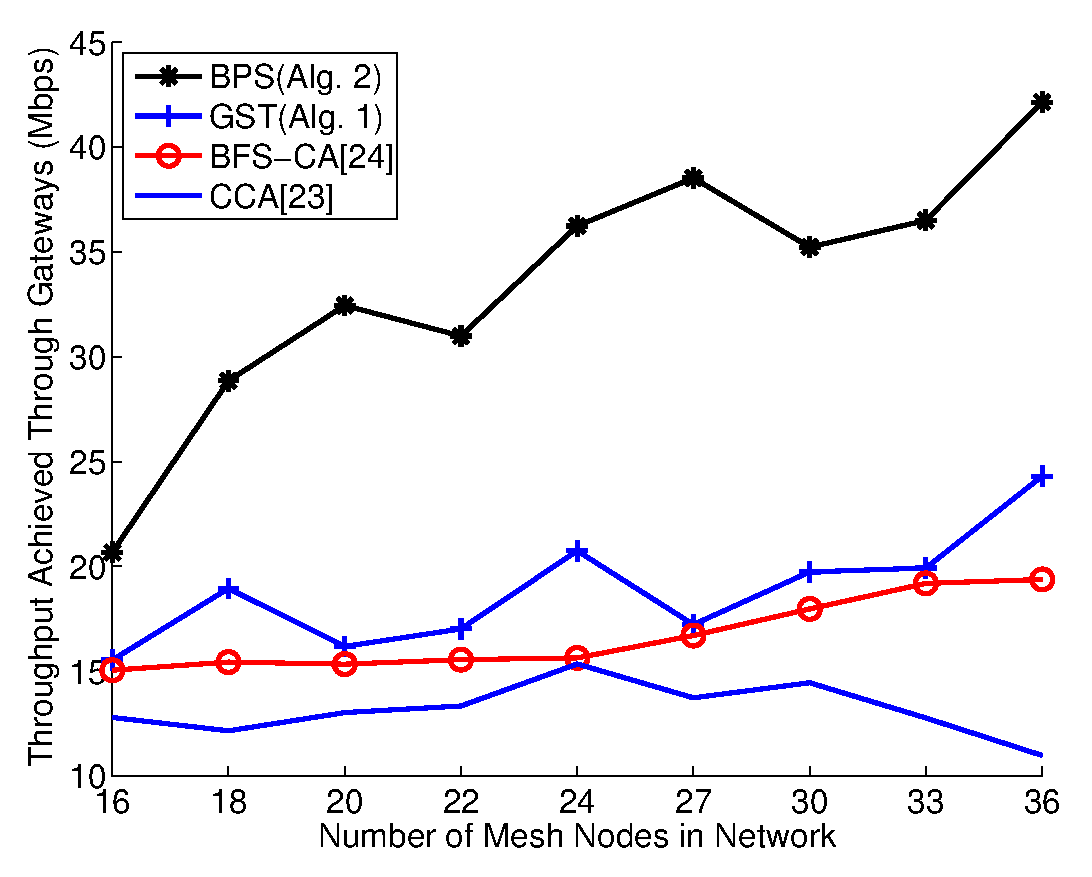
\includegraphics[width=1.6in]{figures/varysize}}
\subfigure[Varying Load, 49-Nodes Regular Grid]{
\label{fig:maxtpt}
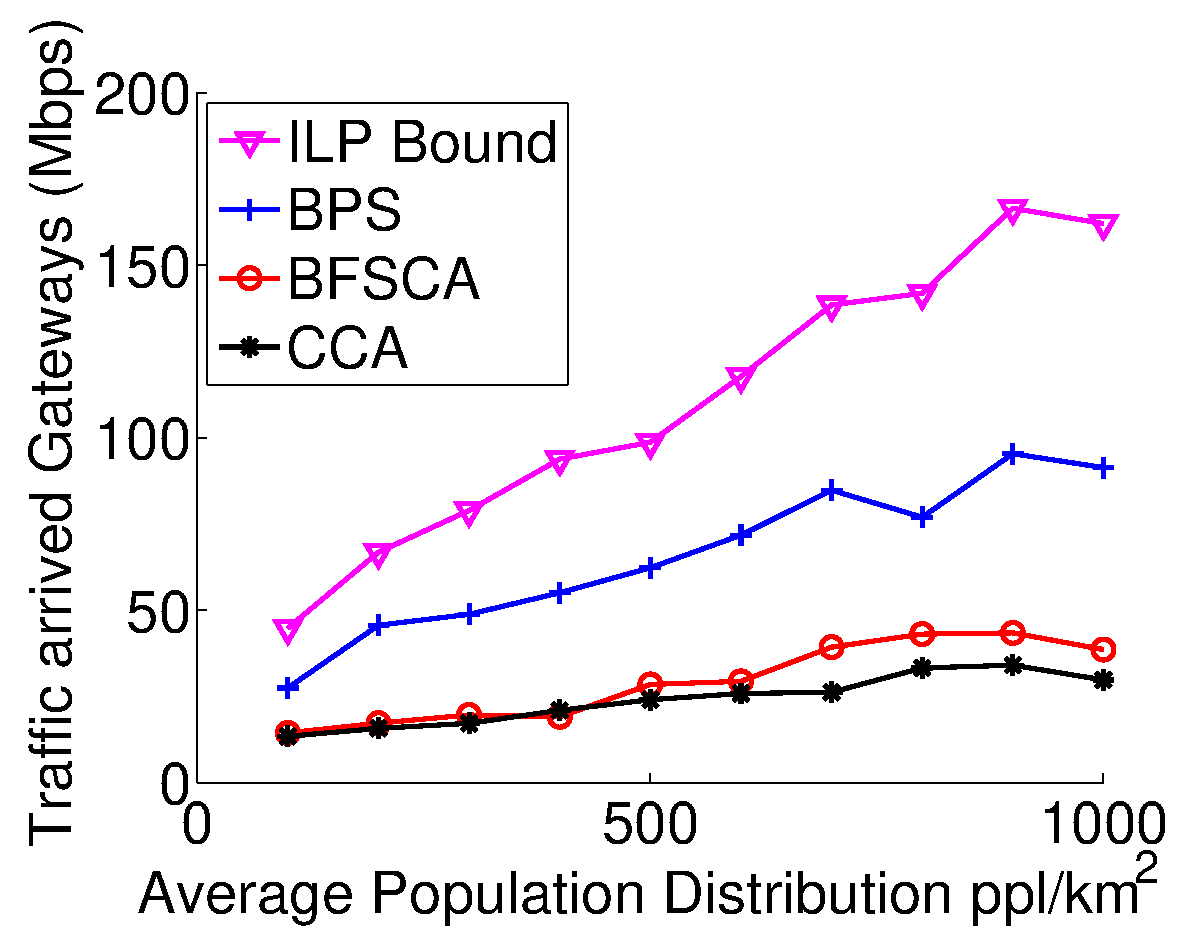
\includegraphics[width=1.6in]{figures/maxtpt.eps}}
\hfill
\caption{Performance in terms of total traffic served for various offered loads, network sizes, and configurations of WiFi or white space (WS) channels.}
\label{fig:all3figs}
\vspace{-0.3in}
\end{figure}
%\end{figure*}

In Fig.~\ref{fig:varysize}, we observe the total traffic served increases with the network size. 
The multiband wireless network has a similar communication and interference performance with 
the multi-channel wireless network with a small network size for all algorithms. 
However, as the network size or population increases, the performance diverges between BPS and 
CCA/BFS-CA.
The nodes of a small network are located in a single interference space of all the bands.
The communication range variation of the bands impact on the network performance when the inter-node spacing become diverse. 
The LP Bound shows the upper-bound of total traffic served increases with the network size.
The multi-channel algorithms assign channels without considering the channel capacity diversity and thepropagation 
differences per band. Hence, the performance 
is remains low across population densities. 
CCA fails to employ the communication range variation to find the most efficient multi hop paths. 
BFS-CA optimizes the first-hop connection from the gateway, but fails to deal the whole path 
from the gateway to destination node. Conversely, BPS alleviates the strain on these first-hop, 
bottleneck links, achieving average 76\% of the LP Bound. The gap of BPS to the LP is partly because 
BPS only considers a fixed multihop path to a gateway node for each access point, whereas the 
LP considers multiple paths to the gateways. For BPS and other heuristic-based algorithms, a dynamic 
assignment version could be implemented through updating the assignment as after path emerge.

\begin{table*}
\centering % centering table 
\begin{tabular}{|c|c|c|c|c|c|c|c|c|c|c|c|} % creating 12 columns 
\hline %\hline % inserting double-line 
%Bands     & \multicolumn{3}{c|}{Dallas} & \multicolumn{3}{c|}{Weatherford} & \multicolumn{3}{c|}{Millsap} \\% [0.5ex]
%\hline % inserts single-line 
% Entering 1st row 
 \multirow{2}{*}{Frequency Bands} & \multicolumn{9}{|c|}{Population Distribution $ppl/km^2$} \\
\cline{2-10}
		& 1500 & 1000 & 500 & 300 &  200 & 150 & 100 & 20 & 10 \\ % [0.5ex]
\hline % inserts single-line 
450 MHz &24.37	&25.83  &23.77	&6.05 &12.50  &14.03 & 7.00 & 0.07 & 0.02 \\      
\hline % inserts single-line                                                                                                       
800 MHz &4.40 	&16.49  &4.77	&5.22&5.07 &4.43  & 3.87 & 4.20 & 3.60 \\      
\hline % inserts single-line                                                                                                      
2.4 GHz &15.87 	&34.95  &2.60	&2.03&2.03 &2.77  & 2.07 & 1.60 & 0.80 \\      
\hline % inserts single-line                                                                                                     
5.2 GHz &19.70	&35.46  &1.53	&1.93&1.93 &1.33  & 1.27 & 2.07 & 2.10 \\      
\hline % inserts single-line 
\end{tabular}    
\caption{Activity Level under Population Distribution} % title name of the table 
\label{tab:activitymeasurement}    
\vspace{-0.3in}
\end{table*}    

% additional Simulation set up
Then we investigate a different form of scalability in our analysis.  Namely,
we increase the average population distribution from 100 to 1,000 per $km^2$, while
maintaining a 49-node regular grid topology. The achieved channel capacity is mapped 
to the spectral analysis with the closest population distribution. 
%
%measurements has the same distance to the current set up, the lower population 
%measurement will be chosen, for instance, we map $400 ppl/km^2$ to $300 ppl/km^2$ 
%measurements as shown in Table.~\ref{tab:activitymeasurement}. 
%
Fig.~\ref{fig:maxtpt} shows the correlation of the population distribution and total traffic served. 
Similar to Fig.~\ref{fig:varysize}, as shown in the figure, the wireless channel capacity of a 
gateway is saturated quickly when the algorithm fails to 
reduce the interference via resource allocation among the channels.
Also, the results show how the achieved channel capacity impacts on the performance. 
As the population density increases, the measurement-based channel capacity varies among multiple 
bands. When the population density reaches 1,000 $ppl$, the total traffic served decreases
due to the high measured activity level and the saturation of wireless channel capacity 
around the gateways. BPS 60\% achieve of the upper bound on average. 
The results shows that CCA and BFS-CA perform worse than BPS with limited recogination of 
propagation variation in the joint WiFi and white space scenarios.

\begin{table*}
\centering % centering table 
\begin{tabular}{|l|c|c|c|c|c|c|c|c|c|c|c|} % creating 12 columns 
\hline %\hline % inserting double-line 
Bands/     & WiFi    & WS      & WS \& & WS \& &  WS \& & WS \& & WS \&      &  WS \&      & Multi-WS \& & Multi-WS \& & Multi-WS \& \\% [0.5ex]
Algorithms & Only    & Only    & WiFi  & WiFi  &  WiFi  & WiFi  & Multi-WiFi &  Multi-WiFi & WiFi        & WiFi        & Multi-WiFi  \\
\hline % inserts single-line 
% Entering 1st row 
WS (MHz)   &                                                        & 450,800 & 450 &  800  &  450   & 800               & 450    & 800      & 450,800     & 450,800     & 450,800     \\
\hline
WiFi (GHz) & 2.4, 5 &                                                             & 2.4 &  2.4  &  5   & 5               & 2.4, 5& 2.4, 5        & 2.4             & 5         & 2.4, 5     \\ % [0.5ex]
\hline
\hline % inserts single-line 
CCA~\cite{draves2004routing}                & 22.4   &  13.4  & 13.2    &12.5    & 16.9       & 23.2   &  24.1  &   30.6&  25.2  &       23.9       &   30.4          \\      
\hline % inserts single-line                                                                                                       
BFS-CA~\cite{ramachandran2006interference}  & 26.3   &  15.8  & 14.9    & 19.4   & 22.7       & 28.4   &  38.9  &   33.7&  30.1  &       27.4       &       36.6      \\      
%\hline % inserts single-line                                                                                                      
%GST (Alg. 1)                                                            & 11.6  &   6.6 & 9.3    &   15.1&   15.8        &  14.4  &   16.6   &    14.1  &   18.8            &  15.0           &    25.1         \\      
\hline % inserts single-line                                                                                                     
BPS (Alg. 1)                                & 41.2   & 34.1   &  38.2  & 40.0    & 35.4       & 42.8   & 58.4   &  64.9 &  54.4  &       51.9       &       63.1      \\      
\hline % inserts single-line 
\end{tabular}    
\caption{ total traffic served (Mbps) for various combinations of WiFi and Average Population Distribution = 500 $ppl/km^2$, Network Size = 49 access points).} % title name of the table 
% NEWClaim fix
\label{tab:2channelcombination}    
\vspace{-0.4in}
\end{table*}    


WhiteMesh networks are able to deploy across a vast array of environments, from
rural to urban areas. Each of these areas will have varying amounts of user
demand traffic in proportion to the population densities. 
However, since a greater number of TV stations exist in urban areas, the available 
white space bands are often inversely related to the population density. 
To capture these varying degrees of demand 
and white space availability we consider three likely scenarios and one final 
scenario for comparison purposes: {\it (i)} two WiFi bands (2.4 and
5.2 GHz) channels with two white space channels (450 and 800 MHz), {\it (ii)} 
three channels in two WiFi bands (2.4 and 5.2 GHz) with one white space channel 
(450 MHz), {\it (iii)} Four channels in two WiFi bands (2.4 and 5.2 GHz) without 
any white space channels, and {\it (iv)} four channels in two white space bands 
(450 and 800 MHz) with no WiFi bands (for comparison).

Table~\ref{tab:2channelcombination} describes the total traffic served 
for various scenarios of WiFi and white space bands with an offered load 
of 5 Mbps as mean value of Possion process from 500 $ppl/km^2$ in a regular 49-node grid. 
We study the performance of BPS in the four aforementioned scenarios of varying 
white space availability. In the simulation, we keep total 4 channels for each
method, such as in the combination of 2.4 GHz and 5 GHz, we put 2 channels in both 
bands. In the triple bands combinations, we set each band has a channel, and put the 
other channel in the highest frequency band. (In 2.4 GHz, 5GHz, 800 MHz combination, 
we put the extra channel other than the 3 channel each band in 5 GHz). 
% Justification
In the results, we observe that the WiFi-only scenario has greater total traffic served 
than the white-space-only scenario. This is due to the lack of spatial reuse achieved 
by white spaces bands. White space has larger communication range to shorten 
the hop counts as well as has larger interference reducing the spatial reuse. 
Another reason is that the achieved channel capacity of 500 $ppl/km^2$ in white 
space bands are worse than WiFi bands. These two reasons make the performance of 
white space only worse in all channel assignment methods applied here.
Interestingly, however, the joint use of both white space and WiFi bands has 
significant gains over the single type of band scenarios with the same number of 
channels (40\% greater than WiFi and 56\% over white space, on average). 

%In 500 $ppl/km^2$ scenario, 5 GHz channel is cleaner than 450 MHz which makes 
%the combination of 2 channels in 5 GHz, 1 channel in 2.4 GHz and 800 MHz has 
%better performance than WiFi(2)+WS(2) in some cases. 


In Table ~\ref{tab:2channelcombination}, that with the same number of bands (2), 
the combination with similar propagation characters, the cleaner channels combination 
has better performance. With similar achieved channel capacity, lower frequency 
offers more option for connection path perform better in channel assignment. 
If we have one channel in a white space band and one channel in a WiFi band, then 
we could employ the advantages of both WiFi for spatial reuse and white spaces to 
reduce the hop count in channel assignment. 

\subsubsection{Access Tier Impacts on Backhaul Tier}

The density of access points increase proportional to the population 
density to offer enough access capacity for the users. 
Hence, the distance among the access points and the channel 
occupancy in backhual tier channel assignment need to be leveraged.
To investigate impacts of the spacing variation and channel occupancy in the access tier 
on the backhaul tier, we perform simulation on a 49-node regular grid WhiteMesh network as
described before. 

In Fig.~\ref{fig:actspac}, we show the impacts of channel occupancy through 
the activity level and spacing variation on wireless white space mesh network. 
In the results, all the bands have the same activity level in the 49-nodes regular 
grid with normalized multiple inter-node spacing 
from 0.2 to 2.1 as discussed in Subsection~\ref{subsec:design}. In the 3-D figure, 
as the activity level increases, the total traffic served decreases due to the reduction 
of achieved channel capacity. In the spatial dimension, when the nodes have extremely
small spacing, lacking the propagation diversity of multiple bands and spacial reuse  make the total traffic served
limited as we have analyzed in Fig~\ref{fig:varysize}. 
While as the spacing gap increases, the high frequency bands
bring higher total traffic served via more spacial reuse. 
As the spacing gap increase, the high frequencies stop communicating due to the limited 
communication range. The number of available channels reductioneleads the total traffic served 
reduce sharply as shown in the figures.

We further study the real world spacing gap variation through BPS with in-field measurements.
We map the largest population distribution in Table~\ref{tab:activitymeasurement} to 
represent the spacing as normalized distance 0.2, and the least population distribution 
as normalized distance 1.7. In a regular grid the spacing distance $D_s$, population 
distribution $P_d$ and access point capacity $M_c$ obey $P_d \cdot \frac{D_s}{2} ^2 \propto M_c$. 
We interpolate activity level for each normalized distance from 0.2 to 1.7 with gap 0.1. 
The results of the heuristic-based algorithms and the results are shown in Fig.~\ref{fig:measurespacing}.

\begin{figure}[t]
\centering
\subfigure[Uniform Activity Level VS. Space Distance]{
\label{fig:actspac}
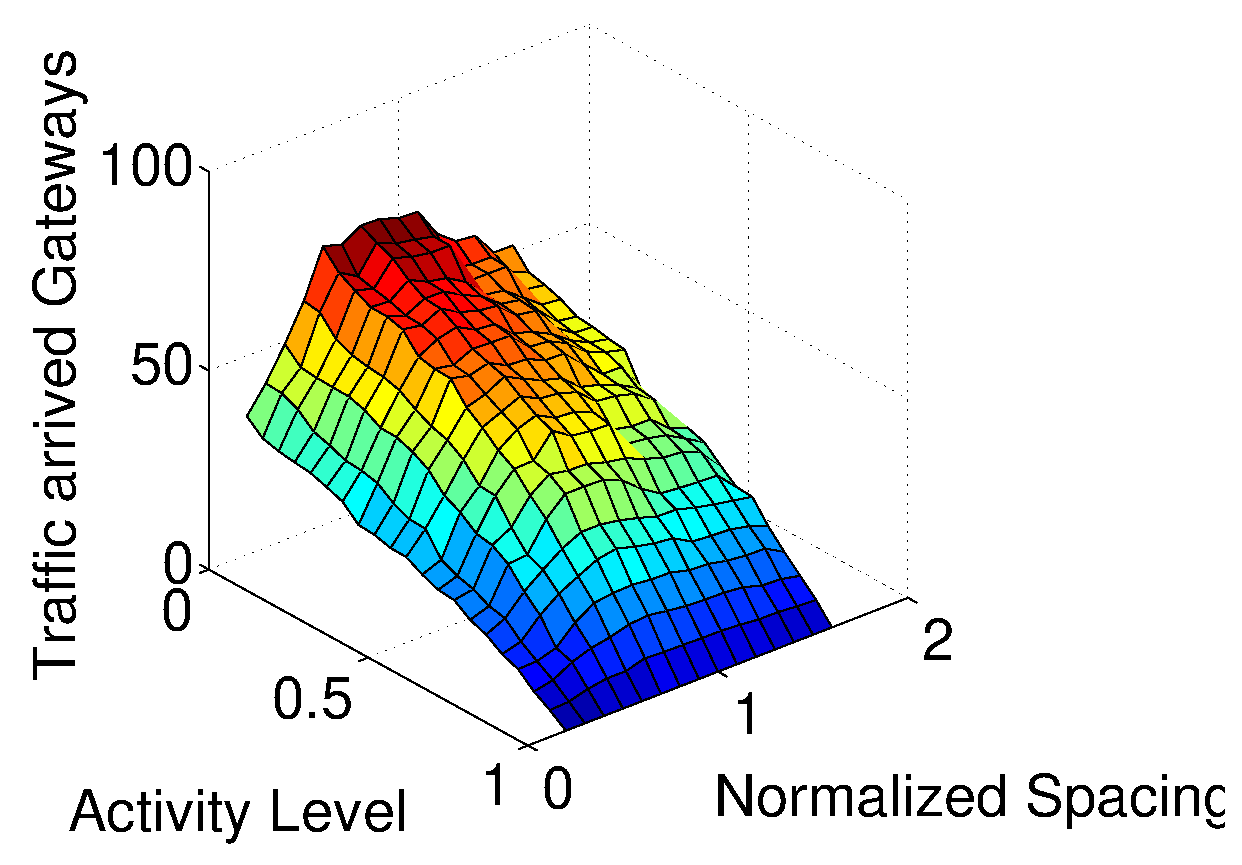
\includegraphics[width=1.6in]{figures/actspac3d}}
\subfigure[total traffic served with Activity Level \& Spacing ]{
\label{fig:measurespacing}
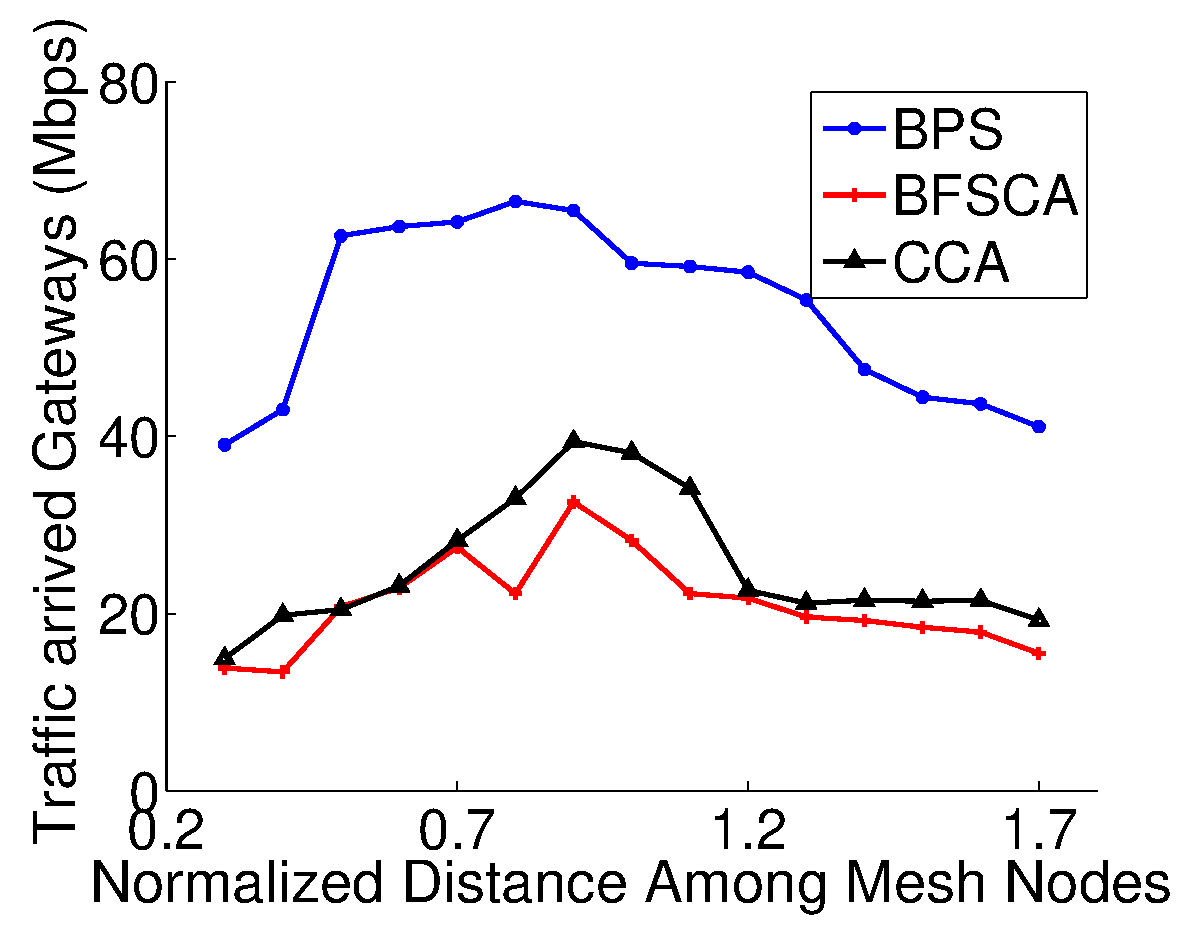
\includegraphics[width=1.6in]{figures/act_spacing}}
\hfill
\caption{Spacing Impacts on the Backhaul Tier}
\label{fig:all3figs}
\vspace{-0.3in}
\end{figure}

In Fig.~\ref{fig:measurespacing}, as the spacing increases, the WhiteMesh network 
has the best performance in all methods through spatial reuse, matching the simulation 
analysis shown in Fig.~\ref{fig:actspac}. As the distance increases up to normalized 
distance 1, one of the 5 GHz channels stops working in the network since the distance 
is larger than its communication range. That makes the performance decrease sharply.

Through these analysis, a mixed WiFi and white space wireless WhiteMesh network 
improves the performance in the following achieve aspects: 
{\it (i)} Heavily utilized networks can get more capacity from spatial reuse and 
flexible path reducing hop count through diverse links. 
{\it (ii)} Rural networks have large mesh spacing to be deployed with a reasonable network performance 
with a fair more reduce of budget.
We are able to find an approaching of optimal WhiteMesh deployment based on this 
analysis.


\section{Related Work}
\label{sec:related}
Since FCC ruling obviated mandatory spectrum sensing in whtie spaces networks, prior research in UHF white spaces has focused on accurate detecting the primary user ~\cite{kim2008fast}; assigning white spaces channels ~\cite{bahl2009white}.
In ~\cite{murty2012senseless}, database is applied to detect white space channel.
Employing the energy advantage of UHF bands is proposed to improve the performance for indoor networks ~\cite{radunovic2010rethinking}.   


In ~\cite{robinson2010deploying}, a placement algorithm for wireless mesh networks is proposed for white space bands.

However, these works only focus on white space bands fails to connect the ISM bands and tons fo existing wireless devices for pratical application.

 %Multichannel works
 Tons of works have been done for multichannel multiradio.

 Cognitive Radios


% Heternegeous networks



 

\section{Conclusion}
\label{sec:conclusion}
In this paper, we exploited the joint use of WiFi and white space bands for 
improving the served user demand of wireless mesh networks.  To do so, we
used an integer programming model to find optimal WhiteMesh topologies.  We
then constructed a heuristic algorithms, Band-based
Path Selection, to achieve similar performance with reduced complexity. Through 
extensive analysis across varying offered loads, network sizes, and white space 
channel availability, we show that our algorithms can achieve 3 to 6 times the served
user demand versus previous multi-channel, multi-radio solutions, since we leverage diverse 
propagation characteristics offered by WiFi and white space bands.  Moreover,
we quantify the degree to which the joint use of these bands can improve the served
user demand. Our BPS algorithm shows that WhiteMesh topologies can achieve up to 
170\% of the gateway goodput of similar WiFi- or white-space-only configurations.
%In future work, we will adapt our algorithms to be used with dynamically-changing
%network conditions, in the field on large-scale WhiteMesh networks.

%investigated the channel assignment in multi-band scenario to leverage the propagation incluence for mesh network applications. 
%We have presented the multi-band mesh network architecture, a new defination of path interference over network, and analyze the advantages and disadvantages of white space bands.
%According to the analysis, we formally propose Best Path Selection and Growing Spanning Tree algorithms for channel assignment in multi-band network. Simulation results show that our scheme outperforms the existing scheme substantially.
%Dynamic and distributed algorithms for multi-band channel assignment problems will be of our future work.



\bibliographystyle{IEEEtran}

\bibliography{whitemesh}

\end{document}
%This is never printed
